\documentclass[11pt,a4paper]{article}

\usepackage[T1]{fontenc}
\usepackage[utf8]{inputenc}
\usepackage{lmodern}
\usepackage{amsmath,amssymb}
\usepackage{booktabs}
\usepackage{tabularx}
\usepackage[section]{placeins}
\usepackage{graphicx}
\usepackage[margin=2.4cm]{geometry}
\usepackage[round,authoryear]{natbib}
\usepackage{caption}
\usepackage{xcolor}
\usepackage[hidelinks]{hyperref}

\graphicspath{{figures/}}
% Generated by eu-okun publication from the committed results. Do not edit.
\makeatletter
\newcommand{\val}[1]{\@ifundefined{okun@#1}{\PackageError{values}{Undefined value #1}{}}{\csname okun@#1\endcsname}}
\expandafter\def\csname okun@by_ES\endcsname{$-0.51$}
\expandafter\def\csname okun@by_ES_ci\endcsname{$[-0.67, -0.30]$}
\expandafter\def\csname okun@by_ES_lagshare\endcsname{$0.22$}
\expandafter\def\csname okun@by_ES_ols\endcsname{$-0.93$}
\expandafter\def\csname okun@by_LU\endcsname{$-0.11$}
\expandafter\def\csname okun@by_LU_ci\endcsname{$[-0.23, +0.01]$}
\expandafter\def\csname okun@by_LU_lagshare\endcsname{$0.57$}
\expandafter\def\csname okun@by_LU_ols\endcsname{$+0.14$}
\expandafter\def\csname okun@by_NL\endcsname{$-0.13$}
\expandafter\def\csname okun@by_NL_ci\endcsname{$[-0.23, -0.04]$}
\expandafter\def\csname okun@by_NL_lagshare\endcsname{$0.94$}
\expandafter\def\csname okun@by_NL_ols\endcsname{$-0.35$}
\expandafter\def\csname okun@by_PT\endcsname{$-0.25$}
\expandafter\def\csname okun@by_PT_ci\endcsname{$[-0.39, -0.12]$}
\expandafter\def\csname okun@by_PT_lagshare\endcsname{$0.58$}
\expandafter\def\csname okun@by_PT_ols\endcsname{$-0.59$}
\expandafter\def\csname okun@by_cov90\endcsname{$94$\%}
\expandafter\def\csname okun@by_factor_corr\endcsname{$-0.60$}
\expandafter\def\csname okun@by_lag1_obs\endcsname{$0.27$}
\expandafter\def\csname okun@by_lag1_p\endcsname{$0.000$}
\expandafter\def\csname okun@by_lag1_rep\endcsname{$0.06$}
\expandafter\def\csname okun@by_mu\endcsname{$-0.198$}
\expandafter\def\csname okun@by_mu_abs\endcsname{$0.20$}
\expandafter\def\csname okun@by_mu_ci\endcsname{$[-0.254, -0.145]$}
\expandafter\def\csname okun@by_mu_hi\endcsname{$-0.18$}
\expandafter\def\csname okun@by_mu_lo\endcsname{$-0.30$}
\expandafter\def\csname okun@by_n_accepted\endcsname{8}
\expandafter\def\csname okun@by_n_neg_all\endcsname{22}
\expandafter\def\csname okun@by_n_neg_linux\endcsname{15}
\expandafter\def\csname okun@by_n_neg_primary\endcsname{24}
\expandafter\def\csname okun@by_n_neg_unpooled\endcsname{15}
\expandafter\def\csname okun@by_n_smaller\endcsname{25}
\expandafter\def\csname okun@by_n_specs\endcsname{9}
\expandafter\def\csname okun@by_pairs_primary\endcsname{99}
\expandafter\def\csname okun@by_pairs_surviving\endcsname{59}
\expandafter\def\csname okun@by_pairs_total\endcsname{351}
\expandafter\def\csname okun@by_rank_width\endcsname{15}
\expandafter\def\csname okun@by_tau\endcsname{$0.126$}
\expandafter\def\csname okun@by_tau_ci\endcsname{$[0.081, 0.175]$}
\expandafter\def\csname okun@by_unpooled_country\endcsname{Slovakia}
\expandafter\def\csname okun@by_unpooled_differ\endcsname{BE, DE, HU, IE, NL, PL and RO}
\expandafter\def\csname okun@by_unpooled_n_differ\endcsname{7}
\expandafter\def\csname okun@by_unpooled_not_ols\endcsname{Belgium and Germany}
\expandafter\def\csname okun@by_unpooled_ols\endcsname{HU, IE, NL, PL and RO}
\expandafter\def\csname okun@by_unpooled_ols_n\endcsname{5}
\expandafter\def\csname okun@by_unpooled_p_hi\endcsname{$0.94$}
\expandafter\def\csname okun@by_unpooled_p_lo\endcsname{$0.73$}
\expandafter\def\csname okun@by_unpooled_rhat\endcsname{$1.0106$}
\expandafter\def\csname okun@cl_ES_excl\endcsname{$-0.79$}
\expandafter\def\csname okun@cl_ES_excl_ci\endcsname{$[-0.99, -0.60]$}
\expandafter\def\csname okun@cl_ES_full\endcsname{$-0.27$}
\expandafter\def\csname okun@cl_ES_full_ci\endcsname{$[-0.39, -0.16]$}
\expandafter\def\csname okun@cl_ES_pre\endcsname{$-0.93$}
\expandafter\def\csname okun@cl_ES_pre_ci\endcsname{$[-1.09, -0.78]$}
\expandafter\def\csname okun@cl_ES_verdict\endcsname{robust negative}
\expandafter\def\csname okun@cl_LU_excl\endcsname{$+0.17$}
\expandafter\def\csname okun@cl_LU_excl_ci\endcsname{$[-0.06, +0.40]$}
\expandafter\def\csname okun@cl_LU_full\endcsname{$-0.05$}
\expandafter\def\csname okun@cl_LU_full_ci\endcsname{$[-0.28, +0.18]$}
\expandafter\def\csname okun@cl_LU_pre\endcsname{$+0.15$}
\expandafter\def\csname okun@cl_LU_pre_ci\endcsname{$[-0.12, +0.43]$}
\expandafter\def\csname okun@cl_LU_verdict\endcsname{sign-unstable}
\expandafter\def\csname okun@cl_NL_excl\endcsname{$-0.28$}
\expandafter\def\csname okun@cl_NL_excl_ci\endcsname{$[-0.43, -0.13]$}
\expandafter\def\csname okun@cl_NL_full\endcsname{$-0.21$}
\expandafter\def\csname okun@cl_NL_full_ci\endcsname{$[-0.26, -0.16]$}
\expandafter\def\csname okun@cl_NL_pre\endcsname{$-0.35$}
\expandafter\def\csname okun@cl_NL_pre_ci\endcsname{$[-0.52, -0.18]$}
\expandafter\def\csname okun@cl_NL_verdict\endcsname{robust negative}
\expandafter\def\csname okun@cl_PT_excl\endcsname{$-0.49$}
\expandafter\def\csname okun@cl_PT_excl_ci\endcsname{$[-0.68, -0.31]$}
\expandafter\def\csname okun@cl_PT_full\endcsname{$-0.13$}
\expandafter\def\csname okun@cl_PT_full_ci\endcsname{$[-0.28, +0.02]$}
\expandafter\def\csname okun@cl_PT_pre\endcsname{$-0.59$}
\expandafter\def\csname okun@cl_PT_pre_ci\endcsname{$[-0.75, -0.42]$}
\expandafter\def\csname okun@cl_PT_verdict\endcsname{negative; significance specification-dependent}
\expandafter\def\csname okun@cl_changed\endcsname{Romania}
\expandafter\def\csname okun@cl_n_attenuated\endcsname{20}
\expandafter\def\csname okun@cl_n_core\endcsname{12}
\expandafter\def\csname okun@cl_n_core_published\endcsname{24}
\expandafter\def\csname okun@cl_n_full_outside\endcsname{10}
\expandafter\def\csname okun@cl_n_neg_excluded\endcsname{22}
\expandafter\def\csname okun@cl_n_neg_holm\endcsname{21}
\expandafter\def\csname okun@cl_n_quarters\endcsname{57}
\expandafter\def\csname okun@cl_n_robust\endcsname{18}
\expandafter\def\csname okun@cl_n_robust_published\endcsname{17}
\expandafter\def\csname okun@cl_pandemic_share_median\endcsname{$78$\%}
\expandafter\def\csname okun@claim_es_holds\endcsname{8}
\expandafter\def\csname okun@claim_es_p\endcsname{$0.996$}
\expandafter\def\csname okun@claim_es_verdict\endcsname{supported}
\expandafter\def\csname okun@claim_lu_holds\endcsname{0}
\expandafter\def\csname okun@claim_lu_p\endcsname{$0.870$}
\expandafter\def\csname okun@claim_lu_verdict\endcsname{not resolved}
\expandafter\def\csname okun@claim_nl_holds\endcsname{6}
\expandafter\def\csname okun@claim_nl_p\endcsname{$0.966$}
\expandafter\def\csname okun@claim_nl_verdict\endcsname{not resolved}
\expandafter\def\csname okun@cs_ES_e_dom\endcsname{$+1.11$}
\expandafter\def\csname okun@cs_ES_e_dom_ci\endcsname{$[+0.78, +1.28]$}
\expandafter\def\csname okun@cs_ES_h\endcsname{$+1.21$}
\expandafter\def\csname okun@cs_ES_h_ci\endcsname{$[+0.97, +1.39]$}
\expandafter\def\csname okun@cs_ES_prod\endcsname{$-0.21$}
\expandafter\def\csname okun@cs_ES_prod_ci\endcsname{$[-0.39, +0.03]$}
\expandafter\def\csname okun@cs_LU_e_dom_pe\endcsname{$+0.03$}
\expandafter\def\csname okun@cs_LU_e_dom_pe_ci\endcsname{$[-0.07, +0.13]$}
\expandafter\def\csname okun@cs_LU_e_res\endcsname{$+0.02$}
\expandafter\def\csname okun@cs_LU_e_res_ci\endcsname{$[-0.05, +0.10]$}
\expandafter\def\csname okun@cs_LU_prod\endcsname{$+1.06$}
\expandafter\def\csname okun@cs_LU_prod_ci\endcsname{$[+0.80, +1.32]$}
\expandafter\def\csname okun@cs_NL_e_dom\endcsname{$+0.46$}
\expandafter\def\csname okun@cs_NL_e_dom_ci\endcsname{$[+0.16, +0.75]$}
\expandafter\def\csname okun@cs_NL_prod\endcsname{$+0.52$}
\expandafter\def\csname okun@cs_NL_prod_ci\endcsname{$[+0.09, +1.05]$}
\expandafter\def\csname okun@cs_PT_dp\endcsname{$+0.18$}
\expandafter\def\csname okun@cs_PT_dp_ci\endcsname{$[+0.09, +0.31]$}
\expandafter\def\csname okun@cs_PT_du\endcsname{$-0.48$}
\expandafter\def\csname okun@cs_PT_du_ci\endcsname{$[-0.64, +0.17]$}
\expandafter\def\csname okun@cs_PT_h\endcsname{$+1.27$}
\expandafter\def\csname okun@cs_PT_h_ci\endcsname{$[+0.93, +1.65]$}
\expandafter\def\csname okun@cs_contradicted\endcsname{0}
\expandafter\def\csname okun@cs_epl_max_n\endcsname{20}
\expandafter\def\csname okun@cs_eplr_by_holm\endcsname{$0.940$}
\expandafter\def\csname okun@cs_eplr_by_n\endcsname{20}
\expandafter\def\csname okun@cs_eplr_by_rho\endcsname{$-0.31$}
\expandafter\def\csname okun@cs_eplr_cl_holm\endcsname{$0.035$}
\expandafter\def\csname okun@cs_eplr_cl_n\endcsname{20}
\expandafter\def\csname okun@cs_eplr_cl_rho\endcsname{$-0.60$}
\expandafter\def\csname okun@cs_eplt_by_holm\endcsname{$0.095$}
\expandafter\def\csname okun@cs_eplt_by_n\endcsname{20}
\expandafter\def\csname okun@cs_eplt_by_rho\endcsname{$-0.54$}
\expandafter\def\csname okun@cs_eplt_noluie_holm\endcsname{$0.020$}
\expandafter\def\csname okun@cs_eplt_noluie_n\endcsname{18}
\expandafter\def\csname okun@cs_eplt_noluie_rho\endcsname{$-0.67$}
\expandafter\def\csname okun@cs_n_corr\endcsname{18}
\expandafter\def\csname okun@cs_n_corr_contra\endcsname{2}
\expandafter\def\csname okun@cs_n_epl\endcsname{6}
\expandafter\def\csname okun@cs_n_epl_decided\endcsname{2}
\expandafter\def\csname okun@cs_n_epl_decided_primary\endcsname{0}
\expandafter\def\csname okun@cs_n_epl_negative\endcsname{6}
\expandafter\def\csname okun@cs_n_indicators\endcsname{6}
\expandafter\def\csname okun@cs_n_pre2020_only\endcsname{2}
\expandafter\def\csname okun@cs_n_pt_unavailable\endcsname{2}
\expandafter\def\csname okun@cs_n_variants\endcsname{3}
\expandafter\def\csname okun@cs_p11\endcsname{$+0.01$}
\expandafter\def\csname okun@cs_p11_ci\endcsname{$[-0.05, +0.05]$}
\expandafter\def\csname okun@cs_p11_holm\endcsname{$1.000$}
\expandafter\def\csname okun@cs_p11_verdict\endcsname{not determined}
\expandafter\def\csname okun@cs_p13\endcsname{$+0.00$}
\expandafter\def\csname okun@cs_p13_ci\endcsname{$[-0.06, +0.05]$}
\expandafter\def\csname okun@cs_p13_holm\endcsname{$1.000$}
\expandafter\def\csname okun@cs_p13_verdict\endcsname{not determined}
\expandafter\def\csname okun@cs_p21a\endcsname{$-0.08$}
\expandafter\def\csname okun@cs_p21a_ci\endcsname{$[-0.60, +0.23]$}
\expandafter\def\csname okun@cs_p21a_holm\endcsname{$1.000$}
\expandafter\def\csname okun@cs_p21a_verdict\endcsname{not determined}
\expandafter\def\csname okun@cs_p22\endcsname{$+0.73$}
\expandafter\def\csname okun@cs_p22_ci\endcsname{$[+0.31, +1.23]$}
\expandafter\def\csname okun@cs_p22_holm\endcsname{$0.022$}
\expandafter\def\csname okun@cs_p22_settings\endcsname{lags-1, pre-2020, block-8}
\expandafter\def\csname okun@cs_p22_verdict\endcsname{supported}
\expandafter\def\csname okun@cs_p23b\endcsname{$-0.22$}
\expandafter\def\csname okun@cs_p23b_ci\endcsname{$[-0.39, -0.06]$}
\expandafter\def\csname okun@cs_p23b_holm\endcsname{$0.100$}
\expandafter\def\csname okun@cs_p23b_verdict\endcsname{not determined}
\expandafter\def\csname okun@cs_p31a\endcsname{$+0.46$}
\expandafter\def\csname okun@cs_p31a_ci\endcsname{$[-0.13, +1.04]$}
\expandafter\def\csname okun@cs_p31a_holm\endcsname{$1.000$}
\expandafter\def\csname okun@cs_p31a_settings\endcsname{pre-2020}
\expandafter\def\csname okun@cs_p31a_verdict\endcsname{not determined}
\expandafter\def\csname okun@cs_p41es\endcsname{$+0.72$}
\expandafter\def\csname okun@cs_p41es_ci\endcsname{$[-1.28, +2.08]$}
\expandafter\def\csname okun@cs_p41es_holm\endcsname{$1.000$}
\expandafter\def\csname okun@cs_p41es_settings\endcsname{pre-2020}
\expandafter\def\csname okun@cs_p41es_verdict\endcsname{not determined}
\expandafter\def\csname okun@cs_p52\endcsname{$-0.06$}
\expandafter\def\csname okun@cs_p52_ci\endcsname{$[-0.51, +0.28]$}
\expandafter\def\csname okun@cs_p52_holm\endcsname{$1.000$}
\expandafter\def\csname okun@cs_p52_verdict\endcsname{not determined}
\expandafter\def\csname okun@cs_pair_ES_LU_h\endcsname{remains}
\expandafter\def\csname okun@cs_pair_ES_NL_h\endcsname{remains}
\expandafter\def\csname okun@cs_pair_ES_PT_h\endcsname{disappears}
\expandafter\def\csname okun@cs_pair_NL_LU_h\endcsname{disappears}
\expandafter\def\csname okun@cs_pairs_disappear\endcsname{2}
\expandafter\def\csname okun@cs_pairs_remain\endcsname{8}
\expandafter\def\csname okun@cs_pairs_reverse\endcsname{0}
\expandafter\def\csname okun@cs_supported\endcsname{1}
\expandafter\def\csname okun@cs_total\endcsname{14}
\expandafter\def\csname okun@dyn_factor_corr\endcsname{$-0.65$}
\expandafter\def\csname okun@dyn_lu_adf\endcsname{holds}
\expandafter\def\csname okun@dyn_lu_adf_p\endcsname{$0.981$}
\expandafter\def\csname okun@dyn_lu_adf_short_p\endcsname{$0.81$}
\expandafter\def\csname okun@dyn_lu_ardl\endcsname{holds}
\expandafter\def\csname okun@dyn_lu_ardl_p\endcsname{$0.995$}
\expandafter\def\csname okun@dyn_mu\endcsname{$-0.17$}
\expandafter\def\csname okun@dyn_mu_ci\endcsname{$[-0.21, -0.13]$}
\expandafter\def\csname okun@dyn_n_neg\endcsname{25}
\expandafter\def\csname okun@dyn_p\endcsname{$0.102$}
\expandafter\def\csname okun@fc_ar1\endcsname{$-1.4$\%}
\expandafter\def\csname okun@fc_ar1_ci\endcsname{$[-3.1, +0.5]$}
\expandafter\def\csname okun@fc_ar1_holm\endcsname{$0.276$}
\expandafter\def\csname okun@fc_ar1_vs_zero\endcsname{$+4.4$\%}
\expandafter\def\csname okun@fc_decided\endcsname{0}
\expandafter\def\csname okun@fc_factor\endcsname{$-5.5$\%}
\expandafter\def\csname okun@fc_factor_ci\endcsname{$[-9.2, -1.9]$}
\expandafter\def\csname okun@fc_factor_holm\endcsname{$0.230$}
\expandafter\def\csname okun@fc_gdp\endcsname{$-15.3$\%}
\expandafter\def\csname okun@fc_gdp_ci\endcsname{$[-25.6, -2.9]$}
\expandafter\def\csname okun@fc_gdp_holm\endcsname{$0.276$}
\expandafter\def\csname okun@fc_origins\endcsname{34}
\expandafter\def\csname okun@fc_total\endcsname{5}
\expandafter\def\csname okun@fc_zero\endcsname{$+4.0$\%}
\expandafter\def\csname okun@fc_zero_ci\endcsname{$[-6.8, +14.7]$}
\expandafter\def\csname okun@fc_zero_holm\endcsname{$1.000$}
\expandafter\def\csname okun@fcx_ar1\endcsname{$-2.9$\%}
\expandafter\def\csname okun@fcx_ar1_holm\endcsname{$0.005$}
\expandafter\def\csname okun@fcx_decided\endcsname{4}
\expandafter\def\csname okun@fcx_factor\endcsname{$-2.5$\%}
\expandafter\def\csname okun@fcx_factor_holm\endcsname{$0.005$}
\expandafter\def\csname okun@fcx_gain_hi\endcsname{$3.1$\%}
\expandafter\def\csname okun@fcx_gain_lo\endcsname{$2.5$\%}
\expandafter\def\csname okun@fcx_gdp\endcsname{$-3.1$\%}
\expandafter\def\csname okun@fcx_gdp_holm\endcsname{$0.005$}
\expandafter\def\csname okun@fcx_holm_max\endcsname{$0.005$}
\expandafter\def\csname okun@fcx_lags\endcsname{$-2.6$\%}
\expandafter\def\csname okun@fcx_lags_holm\endcsname{$0.005$}
\expandafter\def\csname okun@fcx_origins\endcsname{24}
\expandafter\def\csname okun@fcx_total\endcsname{5}
\expandafter\def\csname okun@fcx_zero\endcsname{$-3.5$\%}
\expandafter\def\csname okun@fcx_zero_holm\endcsname{$0.241$}
\expandafter\def\csname okun@gm_contradicted\endcsname{0}
\expandafter\def\csname okun@gm_fin_va_next\endcsname{$10$\%}
\expandafter\def\csname okun@gm_lu_c_q\endcsname{$+0.18$}
\expandafter\def\csname okun@gm_lu_c_y\endcsname{$+0.12$}
\expandafter\def\csname okun@gm_lu_fin_hours\endcsname{$11$\%}
\expandafter\def\csname okun@gm_lu_fin_va\endcsname{$28$\%}
\expandafter\def\csname okun@gm_lu_prod\endcsname{$+1.00$}
\expandafter\def\csname okun@gm_lu_prod_n\endcsname{$+0.95$}
\expandafter\def\csname okun@gm_p11_ie\endcsname{$-0.51$}
\expandafter\def\csname okun@gm_p11_ie_ci\endcsname{$[-0.71, -0.24]$}
\expandafter\def\csname okun@gm_p11_ie_focus\endcsname{$-0.31$}
\expandafter\def\csname okun@gm_p11_ie_holm\endcsname{below 0.001}
\expandafter\def\csname okun@gm_p11_ie_median\endcsname{$+0.19$}
\expandafter\def\csname okun@gm_p11_ie_verdict\endcsname{supported}
\expandafter\def\csname okun@gm_p11_lu\endcsname{$-0.36$}
\expandafter\def\csname okun@gm_p11_lu_ci\endcsname{$[-0.61, -0.02]$}
\expandafter\def\csname okun@gm_p11_lu_focus\endcsname{$-0.17$}
\expandafter\def\csname okun@gm_p11_lu_holm\endcsname{$0.240$}
\expandafter\def\csname okun@gm_p11_lu_median\endcsname{$+0.19$}
\expandafter\def\csname okun@gm_p11_lu_verdict\endcsname{not determined}
\expandafter\def\csname okun@gm_p12_ie\endcsname{$+0.05$}
\expandafter\def\csname okun@gm_p12_ie_ci\endcsname{$[-0.23, +0.40]$}
\expandafter\def\csname okun@gm_p12_ie_focus\endcsname{$+0.41$}
\expandafter\def\csname okun@gm_p12_ie_holm\endcsname{$1.000$}
\expandafter\def\csname okun@gm_p12_ie_median\endcsname{$+0.36$}
\expandafter\def\csname okun@gm_p12_ie_verdict\endcsname{not determined}
\expandafter\def\csname okun@gm_p12_lu\endcsname{$-0.42$}
\expandafter\def\csname okun@gm_p12_lu_ci\endcsname{$[-0.67, -0.09]$}
\expandafter\def\csname okun@gm_p12_lu_focus\endcsname{$-0.06$}
\expandafter\def\csname okun@gm_p12_lu_holm\endcsname{$0.105$}
\expandafter\def\csname okun@gm_p12_lu_median\endcsname{$+0.36$}
\expandafter\def\csname okun@gm_p12_lu_verdict\endcsname{not determined}
\expandafter\def\csname okun@gm_p21_lu\endcsname{$+0.05$}
\expandafter\def\csname okun@gm_p21_lu_ci\endcsname{$[-0.09, +0.20]$}
\expandafter\def\csname okun@gm_p21_lu_focus\endcsname{$+0.05$}
\expandafter\def\csname okun@gm_p21_lu_holm\endcsname{$1.000$}
\expandafter\def\csname okun@gm_p21_lu_median\endcsname{$+0.00$}
\expandafter\def\csname okun@gm_p21_lu_verdict\endcsname{not determined}
\expandafter\def\csname okun@gm_p22_lu\endcsname{$-0.06$}
\expandafter\def\csname okun@gm_p22_lu_ci\endcsname{$[-0.21, +0.10]$}
\expandafter\def\csname okun@gm_p22_lu_focus\endcsname{$-0.05$}
\expandafter\def\csname okun@gm_p22_lu_holm\endcsname{$1.000$}
\expandafter\def\csname okun@gm_p22_lu_median\endcsname{$+0.01$}
\expandafter\def\csname okun@gm_p22_lu_verdict\endcsname{not determined}
\expandafter\def\csname okun@gm_rho_below_ie\endcsname{Sweden}
\expandafter\def\csname okun@gm_rho_dk\endcsname{$-0.22$}
\expandafter\def\csname okun@gm_rho_ee\endcsname{$-0.25$}
\expandafter\def\csname okun@gm_rho_se\endcsname{$-0.35$}
\expandafter\def\csname okun@gm_supported\endcsname{1}
\expandafter\def\csname okun@gm_total\endcsname{8}
\expandafter\def\csname okun@hash_deflator\endcsname{\texttt{30900e56883b8a6e}}
\expandafter\def\csname okun@hash_gdpm\endcsname{\texttt{7cc75f218c9e190d}}
\expandafter\def\csname okun@hash_heterogeneity\endcsname{\texttt{4a6a6d1c82af1e3c}}
\expandafter\def\csname okun@hash_monthly\endcsname{\texttt{ec2e65b6cbe8831f}}
\expandafter\def\csname okun@hash_quarterly\endcsname{\texttt{8a8c8a107d584ba9}}
\expandafter\def\csname okun@hash_shiftshare\endcsname{\texttt{c5c914bb910b1e29}}
\expandafter\def\csname okun@hash_shocks\endcsname{\texttt{8361c685c67770e2}}
\expandafter\def\csname okun@hi_boot_below\endcsname{19}
\expandafter\def\csname okun@hi_bw2_holm\endcsname{6}
\expandafter\def\csname okun@hi_bw8_holm\endcsname{3}
\expandafter\def\csname okun@hi_lost\endcsname{LV and RO}
\expandafter\def\csname okun@hi_negative\endcsname{20}
\expandafter\def\csname okun@hi_negative_holm\endcsname{1}
\expandafter\def\csname okun@hi_over_rejecting\endcsname{23}
\expandafter\def\csname okun@hi_point_negative\endcsname{25}
\expandafter\def\csname okun@hi_rho_gap\endcsname{$+0.17$}
\expandafter\def\csname okun@hi_size_boot\endcsname{$5.1$\%}
\expandafter\def\csname okun@hi_size_normal\endcsname{$22.0$\%}
\expandafter\def\csname okun@hr_above_excl\endcsname{10}
\expandafter\def\csname okun@hr_above_full\endcsname{15}
\expandafter\def\csname okun@hr_d_e_dom\endcsname{$-0.04$}
\expandafter\def\csname okun@hr_d_hpw\endcsname{$+0.34$}
\expandafter\def\csname okun@hr_d_prod\endcsname{$-0.30$}
\expandafter\def\csname okun@hr_mean_du_excl\endcsname{$-0.29$}
\expandafter\def\csname okun@hr_mean_du_full\endcsname{$-0.19$}
\expandafter\def\csname okun@hr_mean_h_excl\endcsname{$+0.43$}
\expandafter\def\csname okun@hr_mean_h_full\endcsname{$+0.74$}
\expandafter\def\csname okun@hr_n_hours\endcsname{26}
\expandafter\def\csname okun@hr_n_no_persons\endcsname{7}
\expandafter\def\csname okun@hr_n_persons\endcsname{20}
\expandafter\def\csname okun@hr_n_settings\endcsname{4}
\expandafter\def\csname okun@hr_no_pandemic\endcsname{$3.3$\%}
\expandafter\def\csname okun@hr_p1\endcsname{$+1.04$}
\expandafter\def\csname okun@hr_p1_amended_ci\endcsname{$[+0.23, +2.08]$}
\expandafter\def\csname okun@hr_p1_amended_holm\endcsname{$0.004$}
\expandafter\def\csname okun@hr_p1_amended_verdict\endcsname{supported}
\expandafter\def\csname okun@hr_p1_ci\endcsname{$[+0.00, +2.21]$}
\expandafter\def\csname okun@hr_p1_holm\endcsname{$0.304$}
\expandafter\def\csname okun@hr_p1_sens_supported\endcsname{4}
\expandafter\def\csname okun@hr_p1_verdict\endcsname{not determined}
\expandafter\def\csname okun@hr_p2a\endcsname{$+0.34$}
\expandafter\def\csname okun@hr_p2a_amended_ci\endcsname{$[+0.05, +0.50]$}
\expandafter\def\csname okun@hr_p2a_amended_holm\endcsname{$0.024$}
\expandafter\def\csname okun@hr_p2a_amended_verdict\endcsname{supported}
\expandafter\def\csname okun@hr_p2a_ci\endcsname{$[+0.00, +0.53]$}
\expandafter\def\csname okun@hr_p2a_holm\endcsname{$0.333$}
\expandafter\def\csname okun@hr_p2a_sens_supported\endcsname{3}
\expandafter\def\csname okun@hr_p2a_verdict\endcsname{not determined}
\expandafter\def\csname okun@hr_p2b\endcsname{$-0.04$}
\expandafter\def\csname okun@hr_p2b_amended_ci\endcsname{$[-0.16, +0.10]$}
\expandafter\def\csname okun@hr_p2b_amended_holm\endcsname{$0.741$}
\expandafter\def\csname okun@hr_p2b_amended_verdict\endcsname{not determined}
\expandafter\def\csname okun@hr_p2b_ci\endcsname{$[-0.16, +0.10]$}
\expandafter\def\csname okun@hr_p2b_holm\endcsname{$0.741$}
\expandafter\def\csname okun@hr_p2b_verdict\endcsname{not determined}
\expandafter\def\csname okun@hr_p3\endcsname{$+0.21$}
\expandafter\def\csname okun@hr_p3_amended_ci\endcsname{$[+nan, +nan]$}
\expandafter\def\csname okun@hr_p3_amended_holm\endcsname{$0.741$}
\expandafter\def\csname okun@hr_p3_amended_verdict\endcsname{not determined}
\expandafter\def\csname okun@hr_p3_ci\endcsname{$[+nan, +nan]$}
\expandafter\def\csname okun@hr_p3_holm\endcsname{$0.741$}
\expandafter\def\csname okun@hr_p3_verdict\endcsname{not determined}
\expandafter\def\csname okun@hr_p_floor\endcsname{$0.067$}
\expandafter\def\csname okun@hr_rank_corr\endcsname{$+0.55$}
\expandafter\def\csname okun@hr_ret_du\endcsname{$0.67$}
\expandafter\def\csname okun@hr_ret_du_ci\endcsname{$[0.56, 1.00]$}
\expandafter\def\csname okun@hr_ret_h\endcsname{$1.70$}
\expandafter\def\csname okun@hr_ret_h_ci\endcsname{$[0.91, 2.99]$}
\expandafter\def\csname okun@hr_towards_du\endcsname{17}
\expandafter\def\csname okun@hr_towards_h\endcsname{6}
\expandafter\def\csname okun@id_max_t\endcsname{$1.27$}
\expandafter\def\csname okun@id_mp_u0\endcsname{$+0.12$}
\expandafter\def\csname okun@id_mp_u0_ci\endcsname{$[+0.03, +0.20]$}
\expandafter\def\csname okun@id_pred_mp\endcsname{$0.580$}
\expandafter\def\csname okun@id_pred_oil\endcsname{$0.006$}
\expandafter\def\csname okun@id_sets\endcsname{4}
\expandafter\def\csname okun@id_unbounded\endcsname{4}
\expandafter\def\csname okun@mo_max_t\endcsname{$1.21$}
\expandafter\def\csname okun@mo_n_direct\endcsname{8}
\expandafter\def\csname okun@mo_pred_oil\endcsname{$0.567$}
\expandafter\def\csname okun@mo_unbounded\endcsname{4}
\expandafter\def\csname okun@n_countries\endcsname{27}
\expandafter\def\csname okun@nr_bh_reg\endcsname{19}
\expandafter\def\csname okun@nr_bh_unres\endcsname{19}
\expandafter\def\csname okun@nr_by_reg\endcsname{1}
\expandafter\def\csname okun@nr_by_unres\endcsname{7}
\expandafter\def\csname okun@nr_holm_block_reg\endcsname{4}
\expandafter\def\csname okun@nr_holm_reg\endcsname{1}
\expandafter\def\csname okun@nr_holm_sieve_reg\endcsname{4}
\expandafter\def\csname okun@nr_holm_unres\endcsname{7}
\expandafter\def\csname okun@nr_size_boot_reg_unres\endcsname{$5.1$\%}
\expandafter\def\csname okun@nr_size_boot_unres\endcsname{$8.0$\%}
\expandafter\def\csname okun@nr_size_normal_unres\endcsname{$16.6$\%}
\expandafter\def\csname okun@nr_ss_bh_reg\endcsname{0}
\expandafter\def\csname okun@nr_ss_bh_unres\endcsname{9}
\expandafter\def\csname okun@nr_ss_by_reg\endcsname{0}
\expandafter\def\csname okun@nr_ss_by_unres\endcsname{0}
\expandafter\def\csname okun@nr_ss_holm_reg\endcsname{0}
\expandafter\def\csname okun@nr_ss_holm_unres\endcsname{0}
\expandafter\def\csname okun@nr_ss_size_boot_reg_unres\endcsname{$4.7$\%}
\expandafter\def\csname okun@nr_ss_size_boot_unres\endcsname{$8.6$\%}
\expandafter\def\csname okun@nr_ss_size_normal_unres\endcsname{$18.1$\%}
\expandafter\def\csname okun@pair_ES_LU\endcsname{survives}
\expandafter\def\csname okun@pair_ES_NL\endcsname{survives}
\expandafter\def\csname okun@pair_ES_PT\endcsname{does not survive}
\expandafter\def\csname okun@pair_LU_NL\endcsname{does not survive}
\expandafter\def\csname okun@pair_LU_PT\endcsname{not supported by either}
\expandafter\def\csname okun@pair_NL_PT\endcsname{not supported by either}
\expandafter\def\csname okun@pc_decided\endcsname{1}
\expandafter\def\csname okun@pc_e1_zero\endcsname{$-13.5$\%}
\expandafter\def\csname okun@pc_e1_zero_holm\endcsname{$0.018$}
\expandafter\def\csname okun@pc_e1_zero_holm_nofail\endcsname{$0.092$}
\expandafter\def\csname okun@pc_e2_ols\endcsname{$-6.7$\%}
\expandafter\def\csname okun@pc_e2_ols_holm\endcsname{$0.061$}
\expandafter\def\csname okun@pc_e2_zero\endcsname{$-0.3$\%}
\expandafter\def\csname okun@pc_e2_zero_holm\endcsname{$1.000$}
\expandafter\def\csname okun@pc_quarters\endcsname{16}
\expandafter\def\csname okun@pc_total\endcsname{10}
\expandafter\def\csname okun@reg_delta\endcsname{$+0.028$}
\expandafter\def\csname okun@reg_delta_ci\endcsname{$[-0.007, +0.072]$}
\expandafter\def\csname okun@reg_tau\endcsname{$0.03$}
\expandafter\def\csname okun@sm_direct_not_average\endcsname{5}
\expandafter\def\csname okun@sm_direct_tie\endcsname{Hungary and Romania}
\expandafter\def\csname okun@sm_lu_auto\endcsname{$-0.51$}
\expandafter\def\csname okun@sm_lu_corr\endcsname{$0.13$}
\expandafter\def\csname okun@sm_misfit_all\endcsname{$+0.27$}
\expandafter\def\csname okun@sm_misfit_direct\endcsname{$+0.26$}
\expandafter\def\csname okun@sm_misfit_smoothed\endcsname{$+0.15$}
\expandafter\def\csname okun@sm_misfit_without\endcsname{$+0.30$}
\expandafter\def\csname okun@sm_n_average\endcsname{10}
\expandafter\def\csname okun@sm_n_smoothed\endcsname{6}
\expandafter\def\csname okun@sm_nl_corr\endcsname{$0.91$}
\expandafter\def\csname okun@sm_p1_direct\endcsname{$+0.26$}
\expandafter\def\csname okun@sm_p1_smoothed\endcsname{$+0.15$}
\expandafter\def\csname okun@sm_p1_verdict\endcsname{not determined}
\expandafter\def\csname okun@sm_p2_direct\endcsname{$+0.62$}
\expandafter\def\csname okun@sm_p2_smoothed\endcsname{$+0.65$}
\expandafter\def\csname okun@sm_p2_verdict\endcsname{not determined}
\expandafter\def\csname okun@sm_smoothed_average\endcsname{0}
\expandafter\def\csname okun@snapshot_date\endcsname{2026-10-15}
\expandafter\def\csname okun@sr_dem_bounded\endcsname{unbounded}
\expandafter\def\csname okun@sr_dem_fevd_hi\endcsname{$96$\%}
\expandafter\def\csname okun@sr_dem_fevd_lo\endcsname{$0$\%}
\expandafter\def\csname okun@sr_dem_gdp8_ci\endcsname{$[-0.06, +1.54]$}
\expandafter\def\csname okun@sr_dem_uniform\endcsname{$-0.43$}
\expandafter\def\csname okun@sr_ls_fevd_hi\endcsname{$96$\%}
\expandafter\def\csname okun@sr_ls_fevd_lo\endcsname{$0$\%}
\expandafter\def\csname okun@sr_n_orderings\endcsname{24}
\expandafter\def\csname okun@sr_nonempty\endcsname{$100$\%}
\expandafter\def\csname okun@sr_nonempty_h01\endcsname{$1.0$\%}
\expandafter\def\csname okun@sr_order_max_h4\endcsname{$-0.202$}
\expandafter\def\csname okun@sr_order_max_h8\endcsname{$-0.216$}
\expandafter\def\csname okun@sr_order_min_h4\endcsname{$-0.135$}
\expandafter\def\csname okun@sr_order_min_h8\endcsname{$-0.149$}
\expandafter\def\csname okun@sr_sets\endcsname{both unbounded}
\expandafter\def\csname okun@sr_tech_bounded\endcsname{unbounded}
\expandafter\def\csname okun@sr_tech_fevd_hi\endcsname{$97$\%}
\expandafter\def\csname okun@sr_tech_fevd_lo\endcsname{$0$\%}
\expandafter\def\csname okun@sr_tech_uniform\endcsname{$-0.55$}
\expandafter\def\csname okun@ss_P1_t\endcsname{$0.19$}
\expandafter\def\csname okun@ss_P2_t\endcsname{$0.31$}
\expandafter\def\csname okun@ss_P3_t\endcsname{$0.66$}
\expandafter\def\csname okun@ss_decision\endcsname{no go}
\expandafter\def\csname okun@ss_published_holm\endcsname{14}
\expandafter\def\csname okun@ss_size_bootstrap\endcsname{$4.8$\%}
\expandafter\def\csname okun@ss_size_normal\endcsname{$22.8$\%}
\expandafter\def\csname okun@ss_survivors\endcsname{0}
\expandafter\def\csname okun@ws_m0_max_t\endcsname{$1.21$}
\expandafter\def\csname okun@ws_m0_unbounded\endcsname{4}
\expandafter\def\csname okun@ws_m1_max_t\endcsname{$1.18$}
\expandafter\def\csname okun@ws_m1_unbounded\endcsname{4}
\expandafter\def\csname okun@ws_q0_max_t\endcsname{$1.27$}
\expandafter\def\csname okun@ws_q0_unbounded\endcsname{4}
\expandafter\def\csname okun@ws_q1_max_t\endcsname{$1.27$}
\expandafter\def\csname okun@ws_q1_unbounded\endcsname{4}
\expandafter\def\csname okun@ws_sr_nonempty\endcsname{$100$\%}
\expandafter\def\csname okun@ws_sr_regions\endcsname{all unbounded}
\makeatother


\setlength{\emergencystretch}{3em}

% Eurostat datasets are cited by their codes.
\defcitealias{eurostat_namq_10_gdp}{\texttt{namq\_10\_gdp}}
\defcitealias{eurostat_une_rt_q}{\texttt{une\_rt\_q}}
\defcitealias{eurostat_lfsi_emp_q}{\texttt{lfsi\_emp\_q}}
\defcitealias{eurostat_une_rt_m}{\texttt{une\_rt\_m}}
\defcitealias{eurostat_sts_inpr_m}{\texttt{sts\_inpr\_m}}
\defcitealias{eurostat_namq_10_pe}{\texttt{namq\_10\_pe}}
\defcitealias{eurostat_namq_10_a10_e}{\texttt{namq\_10\_a10\_e}}
\defcitealias{eurostat_lfsq_etgaed}{\texttt{lfsq\_etgaed}}
\defcitealias{eurostat_lfsq_eegaed}{\texttt{lfsq\_eegaed}}
\defcitealias{eurostat_lfsq_etpga}{\texttt{lfsq\_etpga}}
\defcitealias{eurostat_lfsq_eppga}{\texttt{lfsq\_eppga}}

\newcommand{\E}{\mathbb{E}}
\newcommand{\eu}{EU-27}

\title{Okun's Law in the European Union, 2009--2026:\\
  Association, Prediction and the Limits of Causal Identification}
\author{Diogo Ribeiro}
\date{October 2026}

\begin{document}
\maketitle

\begin{abstract}
\noindent
We re-examine the relation between quarterly real GDP growth and changes in the
unemployment rate in the \val{n_countries} member states of the European Union from 2009
to 2026, using official Eurostat data frozen with cryptographic hashes and analyses
registered before estimation.

\textbf{Association.} With 2020--2021 excluded, the two-lag Okun coefficient sum is
negative, with a 95\% interval below zero, in \val{cl_n_neg_excluded} of
\val{n_countries} countries. Including the pandemic quarters pulls most sums towards zero.
A hierarchical Bayesian model with Student-$t$ errors, residual autocorrelation and a
common European factor gives an unweighted cross-country mean of \val{by_mu} (90\%
interval \val{by_mu_ci}), with a between-country standard deviation of \val{by_tau}.
Country ranks remain highly uncertain.

\textbf{Prediction.} Hierarchical pooling does not improve one-quarter-ahead forecasts
beyond sampling variation, and neither do lagged GDP growth or the common factor: none of
the pre-registered forecast comparisons is decided at the 5\% familywise level.

\textbf{Causation.} External instruments for monetary-policy and oil-supply shocks are weak
for real activity, with first-stage $|t|$ at most \val{id_max_t} quarterly and
\val{mo_max_t} monthly. A foreign-demand shift-share instrument is infeasible (expected
first-stage $t$ of \val{ss_P1_t}). Sign restrictions that the data admit leave the
shock-conditional Okun ratios unbounded.

\textbf{Countries.} We compare the results with three earlier claims: a large association
for Spain, a delayed one for the Netherlands and a weak one for Luxembourg. The Spanish claim
is supported in every accepted specification. The Dutch and Luxembourg claims are not
resolved by their registered rules. In Luxembourg, the data give no sign that the
cross-border measurement mismatch explains the weak association: domestic and resident
employment barely move with GDP, and output per hour absorbs the fluctuations.

Every Okun coefficient in this study is a descriptive association; none is an identified
causal effect.
\end{abstract}

\section{Introduction}\label{sec:intro}

Okun's law is the empirical regularity that unemployment falls when output grows faster
than its trend and rises when it grows more slowly \citep{okun1962}. It is among the most
cited relations in macroeconomics and one of the least settled: its coefficient varies
across countries and periods, and its meaning depends on what moves output in the first
place \citep{ball2017okun}.

\paragraph{Motivation.} This study was prompted by a reported hierarchical Bayesian analysis
of the \eu\ for 2009--2026. That analysis described Spain as having a large association
between GDP growth and unemployment, the Netherlands as having a delayed response, and
Luxembourg as having a weak one, and it suggested measurement and institutional
explanations. We test two explanations of that kind: a mismatch between production by
cross-border commuters and resident unemployment in Luxembourg, and employment
protection. We do not have that analysis's code, data vintage or numerical
estimates. We therefore treat its statements as hypotheses and examine them
independently. The three descriptive claims were written into the protocol of the
Bayesian stage before its estimates, and the two explanations into the protocol of the
case study (Appendix~\ref{app:prereg}). Portugal, about which no claim was made, is
included as a comparison for Spain.

\paragraph{Three questions.} We keep three questions apart throughout.
\begin{enumerate}
  \item \emph{Association.} How large is the conditional association between GDP growth
    and the change in the unemployment rate in each country, and how much do countries
    differ once estimation uncertainty and common European shocks are accounted for?
  \item \emph{Prediction.} Does that association, or the hierarchical pooling of
    countries, improve forecasts of unemployment relative to simple benchmarks?
  \item \emph{Causation.} Can any part of the association be given a structural
    interpretation: the effect on unemployment of an identified shock that moves output?
\end{enumerate}
A large and stable association need not predict well; a useful predictor need not be
causal; and a causal effect of one kind of shock need not equal the reduced-form Okun
coefficient, which averages over all shocks of a period (section~\ref{sec:background}).

\paragraph{Approach.} Each stage was registered before its own estimation, sequentially,
on the same data: its protocol was committed and pushed before it was run, and its change
log records any later clarification with its reason. Later stages were designed knowing
the results of earlier ones (Appendix~\ref{app:prereg}). The data are frozen Eurostat and OECD snapshots
whose raw responses are hashed and re-derived by an audit. Every number in this article is
read by code from the committed result tables (Appendix~\ref{app:repro}). The work
proceeded in stages:
\begin{itemize}
  \item classical regressions and an independent review of them;
  \item a hierarchical Bayesian model with its checks and amendments;
  \item two predictive comparisons;
  \item an identification study with four strategies;
  \item a case study of Portugal, Spain, the Netherlands and Luxembourg.
\end{itemize}

\paragraph{Findings in brief.}
\begin{itemize}
  \item Outside 2020--2021 the two-lag sum is negative in \val{hi_point_negative} of
    \val{n_countries} countries and significantly so in \val{hi_negative} under
    small-sample bootstraps. How many individual sums survive an adjustment for testing
    \val{n_countries} countries depends on the error rate controlled.
  \item Its magnitude depends on the sample, the error model and the treatment of
    persistence, and country rankings are not established.
  \item Over all target quarters, no registered forecast comparison is decided. Without
    the pandemic targets, pooling, GDP lags and the common factor give small gains, but
    nothing reliably beats a forecast of no change.
  \item With the available public data, the instruments and restrictions we could defend
    are uninformative about a causal Okun coefficient.
  \item Of the three earlier claims, Spain's is supported, while the Dutch and Luxembourg
    claims are qualified. The commuter explanation for Luxembourg is not supported. The
    employment-protection correlations all have the opposite sign, but none is decided
    in the primary variant.
\end{itemize}

\paragraph{Outline.} Section~\ref{sec:background} sets out Okun's law and the accounting
identity behind it. Section~\ref{sec:data} describes the data and their measurement
issues. Sections~\ref{sec:classical} and~\ref{sec:bayes} present the classical and
Bayesian methods and estimates. Section~\ref{sec:heterogeneity} turns to uncertainty and
heterogeneity, section~\ref{sec:prediction} to prediction and
section~\ref{sec:identification} to identification. Section~\ref{sec:cases} contains the
country case studies and the comparison with the earlier claims, followed by the
discussion and conclusions. The appendices document reproduction and the pre-registration
record.

\section{Background}\label{sec:background}

\subsection{Two forms of Okun's law}

\citet{okun1962} related the unemployment rate to the gap between actual and potential
output. The \emph{difference} form used here avoids estimating potential output. For
country $i$ and quarter $t$, let $u_{it}$ be the unemployment rate (\% of the labour force),
$\Delta u_{it}=u_{it}-u_{i,t-1}$ its change in percentage points (pp), and $g_{it}$ the
quarter-on-quarter growth of real GDP (\%). Then
\begin{equation}\label{eq:okun}
  \Delta u_{it} = \alpha_i + \sum_{k=0}^{K}\beta_{ik}\, g_{i,t-k} + \varepsilon_{it},
  \qquad \theta_i \equiv \sum_{k=0}^{K}\beta_{ik}.
\end{equation}
The coefficient sum $\theta_i$ is the change in the unemployment rate, in pp, by the end of
quarter $t+K$ that goes with one extra point of growth in quarter $t$ alone, which leaves
the level of output about one per cent higher. Under a sustained one-point rise in quarterly
growth, $\theta_i$ is instead the change in $\Delta u$ per quarter once all lags have
passed, and the cumulative change in the rate keeps growing. $-\alpha_i/\theta_i$ is the
growth rate
consistent with stable unemployment. Lagged growth allows the labour market to respond with
a delay. Estimated coefficients are negative in advanced economies, but their size
differs widely from country to country \citep{ball2017okun}.

\subsection{An accounting identity}

Output $Y$ is the product of output per hour, hours per worker and employment. Employment
$E$ is the labour force $L$ times one minus the unemployment rate. In log changes (lower
case) and with the rate approximation,
\begin{equation}\label{eq:identity}
  g \;\approx\; \underbrace{\Delta\ln(Y/H)}_{\text{productivity}}
  + \underbrace{\Delta\ln(H/E)}_{\text{hours per worker}}
  + \underbrace{\Delta\ln E}_{\text{employment}},
  \qquad
  \Delta u \;\approx\; -(\Delta\ln E - \Delta\ln L).
\end{equation}
An Okun coefficient of $-1$ would require productivity, hours per worker and the labour
force not to move with output. Observed coefficients are much smaller in magnitude because
output fluctuations are absorbed through other margins:
\begin{itemize}
  \item productivity (labour hoarding);
  \item hours per worker (short-time work);
  \item participation, through discouraged or added workers.
\end{itemize}
Institutions shape these margins. Strict dismissal rules combined with flexible temporary
contracts can make employment more volatile \citep{bentolila2012twotier}. Unemployment
inflows and outflows differ widely across countries \citep{blanchard2001portugal}, and
hours per worker vary along the cycle \citep{ohanian2012hours}. The identity also shows
that measurement matters: GDP is a domestic concept (production on the territory), whereas
unemployment and participation describe residents.

\subsection{What a reduced-form coefficient measures}\label{sec:weighted}

Let the reduced-form innovations of $(g,\Delta u)$ be driven by mutually uncorrelated
structural shocks $\varepsilon_k$ (demand, productivity, labour supply, energy, \dots):
\[
  g=\sum_k a_k\varepsilon_k, \qquad \Delta u=\sum_k b_k\varepsilon_k .
\]
Then the regression coefficient of $\Delta u$ on $g$ is
\begin{equation}\label{eq:weighted}
  \beta_{\mathrm{Okun}}=\frac{\operatorname{Cov}(\Delta u,g)}{\operatorname{Var}(g)}
  =\sum_k w_k\,\kappa_k,\qquad
  \kappa_k=\frac{b_k}{a_k},\quad w_k=\frac{a_k^2}{\sum_j a_j^2}.
\end{equation}
The coefficient is a weighted average of shock-conditional Okun coefficients
$\kappa_k$. The weights are each shock's share of output variance, and the same algebra holds
horizon by horizon for cumulative responses. Differences between countries or periods can
therefore reflect different labour-market responses ($\kappa_k$) or different shock
mixes ($w_k$). The data cannot separate the two without identifying the shocks, which is
the subject of section~\ref{sec:identification}. Until then, every coefficient is a
\emph{descriptive association}.

\section{Data and measurement}\label{sec:data}

\subsection{Sources}

All series are official, harmonised and quarterly unless stated otherwise. The core panel
covers the present-day \val{n_countries} member states, from 2008-Q1 (for lags and
differences) to 2026-Q2. It was downloaded from the Eurostat Statistics API on
\val{snapshot_date} and frozen; its manifest has SHA-256 \val{hash_quarterly}\dots.
Table~\ref{tab:data} lists the series; Eurostat datasets are cited by their codes.

\begin{table}[htbp]\centering\small
\caption{Data. SA: seasonally adjusted; SCA: seasonally and calendar adjusted; NSA: not
adjusted. All snapshots are frozen with SHA-256 hashes (Appendix~\ref{app:repro}).}
\label{tab:data}
\footnotesize
\begin{tabularx}{\textwidth}{>{\raggedright\arraybackslash}Xl
  >{\raggedright\arraybackslash}Xl}\toprule
Quantity (unit) & Dataset & Filters & Use \\ \midrule
Real GDP growth (\% q/q) & \citetalias{eurostat_namq_10_gdp} & B1GQ, CLV\_PCH\_PRE, SCA & all \\
Unemployment rate (\% of labour force) & \citetalias{eurostat_une_rt_q} & Y15-74, T, SA & all \\
Participation rate (\% of population) & \citetalias{eurostat_lfsi_emp_q} & ACT, Y15-74, SA & all \\
GDP deflator (\% q/q) & \citetalias{eurostat_namq_10_gdp} & PD\_PCH\_PRE\_NAC, SCA & SVAR \\
Unemployment, monthly (\%) & \citetalias{eurostat_une_rt_m} & TOTAL, SA & monthly LP \\
Industrial production (index) & \citetalias{eurostat_sts_inpr_m} & B-D, SCA, 2021=100 & monthly LP \\
Employment, domestic and resident (persons) & \citetalias{eurostat_namq_10_pe} & EMP\_DC, EMP\_NC, SCA
  & cases \\
Hours worked, total and finance & \citetalias{eurostat_namq_10_a10_e} & TOTAL, K, THS\_HW,
  SCA & cases \\
Value added, total and finance & \citetalias{eurostat_namq_10_a10} & B1G, TOTAL, K,
  CLV20\_MEUR, CP\_MEUR, SCA & cases \\
Temporary employees (persons) & \citetalias{eurostat_lfsq_etgaed} & Y15-74, NSA & cases \\
All employees (persons) & \citetalias{eurostat_lfsq_eegaed} & Y15-74, NSA & cases \\
Temporary and part-time shares (\%) & \citetalias{eurostat_lfsq_etpga}, \citetalias{eurostat_lfsq_eppga} & Y15-74,
  NSA & cases \\
ECB policy surprises (pp) & \citet{jarocinski2020information} & MP\_median (OIS) & LP-IV \\
Oil supply news (\%) & \citet{kanzig2021oil} & surprise series & LP-IV \\
Value added in final demand (USD) & \citet{oecd2025tiva} & FDVA & shift-share \\
Employment protection (index 0--6) & \citet{oecd2020epl} & EPL\_R, EPL\_T, version 3, 2008 & cases \\
\bottomrule\end{tabularx}
\end{table}

\subsection{Measurement issues}

\paragraph{Domestic and resident concepts.} GDP measures production by resident
producer units, including work by cross-border commuters. Unemployment and participation
describe residents. The two diverge most in Luxembourg, where commuters fill a large share
of domestic jobs; section~\ref{sec:cases} tests whether this explains Luxembourg's weak
association.

\paragraph{Survey changes.} The EU Labour Force Survey changed its legal framework in 2021.
Eurostat back-casts the headline series from 2009, but:
\begin{itemize}
  \item Spain and France are flagged ``definition differs'' from 2021-Q1, because they still
    test workers on temporary lay-off under the earlier rule;
  \item the Netherlands phased the new survey in during 2021 without a flag;
  \item detailed survey series carry breaks, for example at 2014-Q1 and 2021-Q1.
\end{itemize}
Eurostat's quality flags are stored with every observation. The Bayesian models mask
likelihood terms that rely on a flagged value. The classical review uses a
flag-screened sample as a sensitivity analysis.

\paragraph{Monthly unemployment.} Eurostat's monthly unemployment rate is a direct
monthly survey estimate in only eight countries. Elsewhere it is a trend, a three-month
moving average, or quarterly survey results interpolated with registered unemployment.
Each of these puts later months into a month's value. Section~\ref{sec:identification}
therefore restricts the monthly analysis to the eight direct-estimate countries.

\paragraph{The pandemic.} The eight quarters of 2020--2021 contain the largest movements
of GDP in the sample. Across countries, they supply a median
\val{cl_pandemic_share_median} of the variation in current-quarter GDP growth in the full
sample. Large output movements were also met by job-retention schemes that kept workers
employed. Any estimate that includes 2020--2021 mainly describes the pandemic, so we
report samples with and without it and make the choice explicit in each protocol.

\paragraph{Revisions and timing.} Every series is a revised vintage. Eurostat's vintage
datasets cover GDP only for the EU and euro-area aggregates, and monthly unemployment only
from 2021, so the forecasts in section~\ref{sec:prediction} are retrospective
(pseudo-out-of-sample), not real-time.

\section{Classical estimates}\label{sec:classical}

\subsection{Method}

For each country, equation~\eqref{eq:okun} is estimated by ordinary least squares. Lag
orders are $K\in\{0,1,2,4\}$, with and without the change in the participation rate as a
control. The headline specification is $K=2$ without participation.

\paragraph{Inference.} Standard errors use the Newey--West covariance with a Bartlett
kernel and four lags in calendar quarters \citep{newey1987hac}. The variance of
$\hat\theta_i$ uses the full covariance matrix of the lag coefficients.

\paragraph{Samples.} The full period, 2009--2026; the same period without any observation
whose window touches 2020--2021; 2009--2019; 2022 onwards; and a flag-screened sample.

\paragraph{Review.} A separate review recomputed every published quantity by an
independent numerical route and re-estimated 24 core specifications per country. It
classified each country as robustly negative, negative with specification-dependent
significance, or sign-unstable.

\subsection{Results}

\paragraph{The association.} With 2020--2021 excluded, the two-lag sum is negative with a
95\% interval below zero in \val{cl_n_neg_excluded} of \val{n_countries} countries
(table~\ref{tab:countries}). In \val{cl_n_robust} countries every core specification agrees
in sign and excludes zero. These are associations conditional on contemporaneous and
lagged GDP growth. Contemporaneous growth is not exogenous, and the participation control
can absorb part of the association, a ``bad control'' in the sense of a variable that is
itself an outcome.

\paragraph{The pandemic.} Including 2020--2021 moves the sum towards zero in
\val{cl_n_attenuated} countries (figure~\ref{fig:pandemic}). In \val{cl_n_full_outside}
countries the full-sample estimate lies outside the 95\% interval of the estimate without
the pandemic. The pandemic quarters combine the largest output movements of the sample
with job-retention schemes that kept unemployment from following output. The full-sample
coefficient therefore describes those quarters, not the 2009--2019 relationship.

\paragraph{Post-2021 stability.} The original classical analysis tested whether the sum
changed after 2021 with interacted HAC regressions and Holm's step-down adjustment
\citep{holm1979}; \val{ss_published_holm} changes were significant. With only about
seventeen post-2021 quarters, however, the asymptotic normal reference is unreliable. A
pre-registered study replaced it with null-imposed sieve and moving-block bootstraps of the
same statistic \citep{kunsch1989bootstrap}:
\begin{itemize}
  \item \val{ss_survivors} of the \val{ss_published_holm} published changes survive;
  \item a size study under each test's fitted null shows why: the nominal 5\% normal test
    rejects \val{ss_size_normal} of the time, whereas the bootstrap test rejects
    \val{ss_size_bootstrap}.
\end{itemize}
A weaker association after 2021 is therefore a descriptive pattern, not a tested result.
The Bayesian regime models (section~\ref{sec:bayes}) agree.

% Generated by eu-okun publication. Do not edit.
\begin{table}[htbp]\centering\small
\caption{Two-lag sums $\theta_i=\sum_{k=0}^{2}\beta_{ik}$ (pp of unemployment-rate change per pp of quarterly GDP growth). Classical: OLS on the full sample and without 2020--2021; the interval is the small-sample bootstrap-$t$ 95\% interval of the Newey--West statistic (normal intervals over-reject with this few quarters). $^{*}$ significantly negative under both registered bootstraps; $^{**}$ also after the registered Holm adjustment. Bayesian: posterior median and 90\% credible interval of the primary hierarchical model (2009--2019). Verdict over the core grid without the participation control (normal intervals): robust negative (robust), negative with specification-dependent significance (spec.-dep.), or sign-unstable. Alphabetical; no ranking is implied. Descriptive associations. The original review, which also counted participation-controlled specifications, classed RO as spec.-dep.}
\label{tab:countries}
\begin{tabular}{lrrrl}
\toprule
Country & Full sample & Without 2020--21 [bootstrap 95\%] & Bayes median [90\%] & Verdict \\
\midrule
AT & $-0.23$ & $-0.21^{*}$ $[-0.37, -0.05]$ & $-0.18$ $[-0.30, -0.07]$ & robust \\
BE & $-0.03$ & $-0.14$ $[-0.75, +0.45]$ & $-0.24$ $[-0.40, -0.08]$ & spec.-dep. \\
BG & $-0.33$ & $-0.41^{*}$ $[-0.69, -0.14]$ & $-0.17$ $[-0.31, -0.03]$ & robust \\
CY & $-0.27$ & $-0.47^{*}$ $[-0.68, -0.26]$ & $-0.25$ $[-0.36, -0.13]$ & robust \\
CZ & $-0.19$ & $-0.27^{*}$ $[-0.38, -0.17]$ & $-0.17$ $[-0.24, -0.09]$ & robust \\
DE & $-0.10$ & $-0.18^{*}$ $[-0.30, -0.05]$ & $-0.11$ $[-0.18, -0.05]$ & robust \\
DK & $-0.18$ & $-0.14$ $[-0.53, +0.24]$ & $-0.19$ $[-0.31, -0.07]$ & spec.-dep. \\
EE & $-0.46$ & $-0.49^{**}$ $[-0.71, -0.28]$ & $-0.32$ $[-0.47, -0.18]$ & robust \\
EL & $-0.40$ & $-0.62^{*}$ $[-0.84, -0.40]$ & $-0.37$ $[-0.48, -0.23]$ & robust \\
\textbf{ES} & $-0.27$ & $-0.79^{*}$ $[-1.15, -0.45]$ & $-0.51$ $[-0.67, -0.30]$ & robust \\
FI & $-0.28$ & $-0.24^{*}$ $[-0.36, -0.12]$ & $-0.20$ $[-0.30, -0.10]$ & robust \\
FR & $-0.00$ & $-0.30^{*}$ $[-0.49, -0.12]$ & $-0.20$ $[-0.30, -0.10]$ & sign-unstable \\
HR & $-0.16$ & $-0.47^{*}$ $[-0.84, -0.09]$ & $-0.27$ $[-0.44, -0.12]$ & spec.-dep. \\
HU & $-0.13$ & $-0.18^{*}$ $[-0.30, -0.06]$ & $-0.16$ $[-0.25, -0.06]$ & robust \\
IE & $-0.06$ & $-0.07^{*}$ $[-0.13, +0.00]$ & $-0.06$ $[-0.11, -0.02]$ & robust \\
IT & $-0.04$ & $-0.51^{*}$ $[-0.80, -0.22]$ & $-0.32$ $[-0.50, -0.15]$ & spec.-dep. \\
LT & $-0.36$ & $-0.45^{*}$ $[-0.81, -0.08]$ & $-0.24$ $[-0.36, -0.11]$ & robust \\
\textbf{LU} & $-0.05$ & $+0.17$ $[-0.06, +0.40]$ & $-0.11$ $[-0.23, +0.01]$ & sign-unstable \\
LV & $-0.32$ & $-0.37$ $[-0.81, +0.08]$ & $-0.27$ $[-0.38, -0.14]$ & robust \\
MT & $-0.09$ & $-0.01$ $[-0.07, +0.04]$ & $-0.04$ $[-0.09, +0.00]$ & spec.-dep. \\
\textbf{NL} & $-0.21$ & $-0.28^{*}$ $[-0.51, -0.05]$ & $-0.13$ $[-0.23, -0.04]$ & robust \\
PL & $-0.09$ & $-0.24^{*}$ $[-0.40, -0.08]$ & $-0.13$ $[-0.21, -0.06]$ & robust \\
\textbf{PT} & $-0.13$ & $-0.49^{*}$ $[-0.82, -0.18]$ & $-0.25$ $[-0.39, -0.12]$ & spec.-dep. \\
RO & $-0.11$ & $-0.07$ $[-0.15, +0.02]$ & $-0.05$ $[-0.09, -0.00]$ & robust \\
SE & $-0.22$ & $-0.22^{*}$ $[-0.41, -0.02]$ & $-0.17$ $[-0.25, -0.11]$ & robust \\
SI & $-0.18$ & $-0.25^{*}$ $[-0.47, -0.02]$ & $-0.15$ $[-0.26, -0.04]$ & robust \\
SK & $-0.13$ & $+0.04$ $[-0.85, +0.91]$ & $-0.09$ $[-0.20, +0.01]$ & sign-unstable \\
\bottomrule
\end{tabular}
\end{table}


\begin{figure}[t]\centering
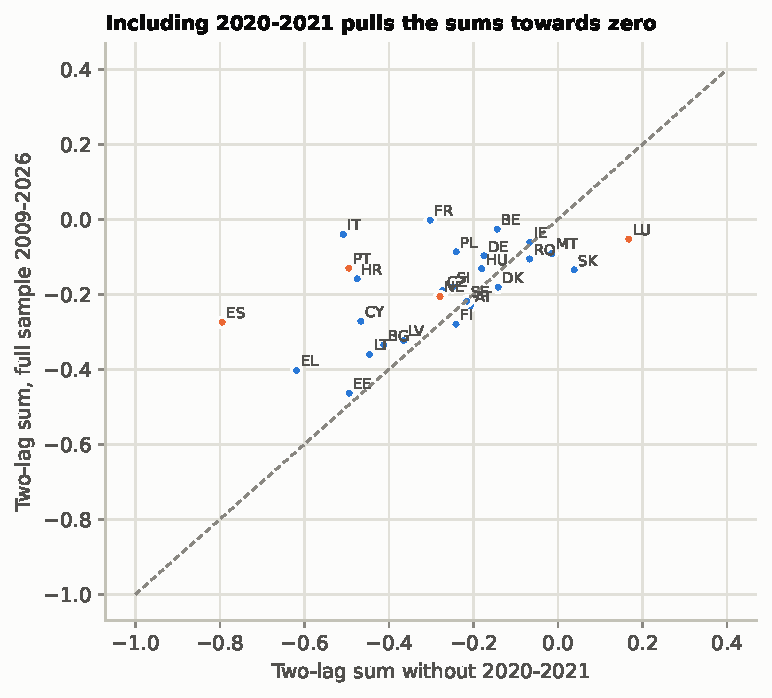
\includegraphics[width=0.62\textwidth]{fig2_pandemic.pdf}
\caption{Classical two-lag sums ($K=2$): full sample (vertical) against the sample without
2020--2021 (horizontal). For negative sums, a point above the diagonal is closer to zero
when the pandemic quarters are included. Focus countries in orange.}\label{fig:pandemic}
\end{figure}

\section{Hierarchical Bayesian estimates}\label{sec:bayes}

\subsection{Model}

The primary model keeps $\theta_i$ as the coefficient sum but lets countries borrow
strength from one another, and it models the dependence that the classical regressions
leave in the residuals. Write $y_{it}=\Delta u_{it}$ and reparameterise the lag weights so
that $\theta_i$ appears directly:
\begin{align}
  y_{it} &= \alpha_i + \theta_i\, g_{it} + \sum_{k=1}^{K} b_{ik}\,(g_{i,t-k}-g_{it})
            + \lambda_i f_t + e_{it}, \label{eq:bayes}\\
  e_{it} &= \phi_i\, e_{i,t-1} + \sigma_i\,\eta_{it},\qquad \eta_{it}\sim t_\nu ,
\end{align}
with $K=2$. Here:
\begin{itemize}
  \item $f_t\sim N(0,1)$ is a common quarterly factor with non-negative loadings
    $\lambda_i$, representing European shocks not captured by each country's own growth;
  \item the AR(1) term captures residual persistence;
  \item Student-$t$ innovations allow for outlying quarters.
\end{itemize}
Country parameters are partially pooled \citep{gelman2013bda} through non-centred
hierarchies, for example
$\theta_i=\mu_\theta+\tau_\theta z_i$ with $z_i\sim N(0,1)$. Analogous hierarchies apply
to $\alpha_i$, $b_{ik}$, $\phi_i$ (on the $\tanh$ scale) and $\log\sigma_i$.

\paragraph{Priors.} The prior on the mean sum, $\mu_\theta\sim N(0,0.5^2)$, is centred at
zero, so the prior does not assume Okun's law. The other priors are
$\tau_\theta\sim N^+(0,0.25^2)$, $\lambda_i\sim N^+(0,0.2^2)$ and
$\nu\sim\mathrm{Gamma}(2,0.1)$. Prior predictive checks show that these weakly informative
priors put visible mass on implausibly large quarterly changes. This is reported rather
than tuned.

\paragraph{Estimands.} $\mu_\theta$ is the mean of the population distribution of country
sums: an unweighted cross-country average. It is not an EU aggregate and not a pooled
slope. With the common factor in the model, $\theta_i$ measures the association with each
country's GDP growth beyond the common European cycle.

\paragraph{Sample.} The primary sample is 2009-Q2 to 2019-Q4: the longest window that is
contiguous and definition-consistent in every country.

\subsection{Posterior inference}

\paragraph{Sampler.} Posteriors are sampled with the No-U-Turn sampler
\citep{hoffman2014nuts} in NumPyro \citep{phan2019numpyro}: four chains of 1000 warm-up and
1000 retained draws, target acceptance $0.95$, fixed seeds.

\paragraph{Acceptance.} A fit is accepted only if all four conditions hold:
\begin{itemize}
  \item the rank-normalised $\widehat R\le 1.01$ \citep{vehtari2021rhat};
  \item bulk and tail effective sample sizes are at least 400;
  \item there are no divergences;
  \item E-BFMI $\ge 0.3$.
\end{itemize}
A failed fit is reported and not interpreted.

\paragraph{Sensitivity.} Nine specifications were fixed in advance: wide priors, strong
pooling, no pooling, no common factor, Gaussian i.i.d.\ errors, the participation control,
four lags, and a sample without 2020--2021. Of these, \val{by_n_accepted} of
\val{by_n_specs} were accepted; the unpooled fit missed the $\widehat R$ threshold.

\paragraph{Model comparison and checks.} Models are compared by PSIS-LOO
\citep{vehtari2017loo} and checked with posterior predictive statistics.

\subsection{Results}

\paragraph{Average and spread.} The mean country sum is $\mu_\theta=$ \val{by_mu} (90\%
credible interval \val{by_mu_ci}). The between-country standard deviation is
$\tau_\theta=$ \val{by_tau} (\val{by_tau_ci}).

\paragraph{Country signs.}
\begin{itemize}
  \item \val{by_n_neg_primary} of \val{n_countries} country sums are credibly negative,
    meaning $P(\theta_i<0)\ge 0.95$, in the primary fit;
  \item \val{by_n_neg_all} are credibly negative in every accepted specification.
\end{itemize}

\paragraph{Magnitudes.} The Bayesian sums are smaller in magnitude than OLS on the same
quarters in \val{by_n_smaller} of \val{n_countries} countries (table~\ref{tab:countries},
figure~\ref{fig:countries}). Pooling
explains only part of the difference. The error model and the common factor change the
estimand: the classical sum includes the common cycle, while the factor model's sum does
not.

\paragraph{Checks.} The posterior predictive checks find one systematic misfit:
\begin{itemize}
  \item the lag-1 autocorrelation of unemployment changes is \val{by_lag1_obs} in the data
    but \val{by_lag1_rep} on average in replicated data, so the primary model understates
    persistence;
  \item central 90\% one-step predictive intervals cover \val{by_cov90} of observations.
\end{itemize}

\paragraph{Amendments.} A registered amendment added an AR(1) common factor and lagged
unemployment changes. Their combination removes the persistence misfit (posterior
predictive $p=$ \val{dyn_p}) and is preferred by PSIS-LOO. Its factor remains correlated
with average GDP growth (\val{dyn_factor_corr}). A second amendment allowed the coefficient
sums to shift after 2021: the average shift is \val{reg_delta} (\val{reg_delta_ci}), with no
credible change in any evaluable country.

\begin{figure}[t]\centering
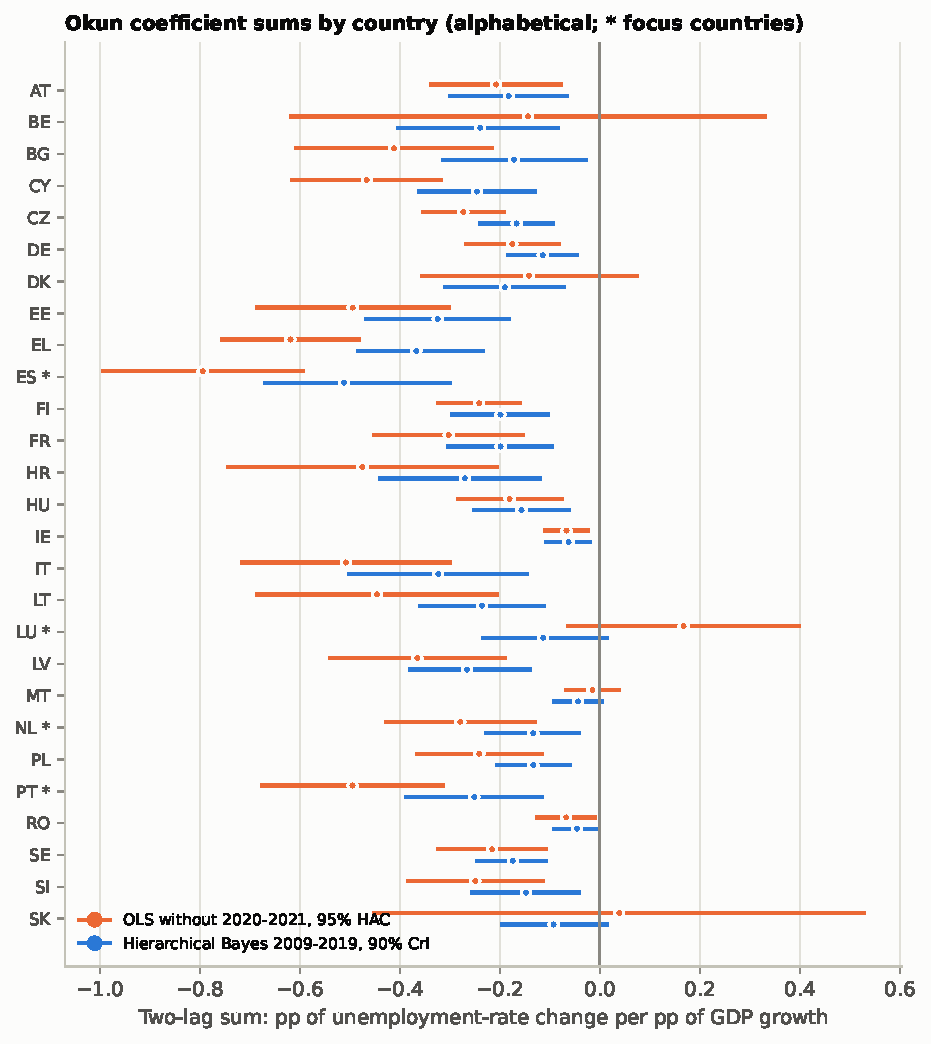
\includegraphics[width=0.78\textwidth]{fig1_countries.pdf}
\caption{Two-lag sums by country. Orange: OLS without 2020--2021 with 95\% HAC intervals.
Blue: hierarchical Bayesian posterior median, 2009--2019, with 90\% credible intervals.
Alphabetical order; focus countries marked. The Bayesian estimand excludes the common
European factor, so the two are not expected to coincide.}\label{fig:countries}
\end{figure}

\section{Uncertainty and country heterogeneity}\label{sec:heterogeneity}

\paragraph{Ranks are not established.} Because estimates are uncertain and correlated
through common shocks, rankings of point estimates are not informative. The posterior
distribution of each country's rank is wide: in the primary fit, the median width of the
90\% rank interval is \val{by_rank_width} of \val{n_countries} places. No country's position
in an ordering of Okun coefficients is established, and none is reported.

\paragraph{Pairwise differences.} A difference between two countries is credible if
$P(\theta_i<\theta_j)\ge 0.95$ or $\le 0.05$.
\begin{itemize}
  \item In the primary fit, \val{by_pairs_primary} of \val{by_pairs_total} pairs differ
    credibly.
  \item Only \val{by_pairs_surviving} pairs are credible in every accepted specification of
    the registered sensitivity set.
  \item Much of the apparent heterogeneity therefore depends on modelling choices.
\end{itemize}

\paragraph{The focus pairs.} Each pair gets one of three verdicts:
\emph{survives} (credible in the same direction in every accepted fit), \emph{does not
survive} (apparent in the classical comparison but not credible in every fit), or
\emph{not supported by either} (neither the classical comparison nor the posterior
supports it).
\begin{itemize}
  \item Spain--Luxembourg: \val{pair_ES_LU}.
  \item Spain--Netherlands: \val{pair_ES_NL}.
  \item Spain--Portugal: \val{pair_ES_PT}.
  \item Luxembourg--Netherlands: \val{pair_LU_NL}.
  \item Luxembourg--Portugal: \val{pair_LU_PT}.
  \item Netherlands--Portugal: \val{pair_NL_PT}.
\end{itemize}

\paragraph{Two sources of heterogeneity.} Equation~\eqref{eq:weighted} gives two reasons why
countries can differ:
\begin{itemize}
  \item labour markets may respond differently to the same shock;
  \item countries may face different mixes of shocks.
\end{itemize}
The estimates in this section cannot separate the two. Section~\ref{sec:cases} asks a
narrower question that the data can address: through which margins of the accounting
identity~\eqref{eq:identity} output fluctuations are absorbed in four countries.

\section{Predictive evaluation}\label{sec:prediction}

A coefficient can describe the data well without improving forecasts. Two pre-registered
comparisons asked whether it does. Both refit every model at every origin, on data strictly
before the target.

\subsection{Designs}

\paragraph{Conditional prediction.} The first design predicts $\Delta u_{i,t}$ given all
data up to $t-1$ \emph{and} the GDP growth of quarter $t$, the setting the Okun equations
describe. There are two evaluation sets, each of \val{pc_quarters} target quarters:
2016--2019 (E1)
and 2022-Q3 to 2026-Q2 (E2). Five models are compared:
\begin{itemize}
  \item the hierarchical Bayesian model;
  \item its Gaussian i.i.d.\ variant;
  \item the OLS distributed lag;
  \item an ARDL model;
  \item a zero-change benchmark.
\end{itemize}

\paragraph{One-quarter-ahead forecasts.} The second design issues the forecast for quarter
$t$ at the end of $t-1$ and uses nothing dated $t$. There are \val{fc_origins} origins,
with targets from
2018-Q1 to 2026-Q2. It compares:
\begin{itemize}
  \item six classical models: persistence (a forecast of zero change), the historical mean, AR(1) of the change, two
    GDP lags, AR(1) with GDP lags, and that model with lagged participation;
  \item three hierarchical Bayesian forecasting models: an AR(1), AR(1) with GDP lags, and
    the same with a common factor.
\end{itemize}
The data are revised vintages, so the forecasts are retrospective, not real-time
(section~\ref{sec:data}).

\paragraph{Scoring.} Predictive distributions are scored with the continuous ranked
probability score (CRPS), a strictly proper scoring rule \citep{gneiting2007scoring}:
\[
  \mathrm{CRPS}(F,y)=\int_{-\infty}^{\infty}\big(F(z)-\mathbf 1\{z\ge y\}\big)^2\,dz .
\]
Scores are averaged over countries within each quarter, so that cross-country dependence is
handled at the level of quarters.

\paragraph{Inference.} The two designs use different procedures:
\begin{itemize}
  \item \emph{Conditional:} a Diebold--Mariano test on the quarterly mean differentials
    \citep{diebold1995accuracy}, with the small-sample correction of
    \citet{harvey1997dm};
  \item \emph{Forecasts:} a synchronised circular block bootstrap over target quarters.
\end{itemize}
Each family of pre-registered comparisons is Holm-adjusted.

\subsection{Results}

Each result below is the mean CRPS of the first model relative to the second; a negative
value favours the first.

\paragraph{Conditional prediction.} Decided comparisons: \val{pc_decided} of
\val{pc_total} (table~\ref{tab:predictive}, figure~\ref{fig:prediction}).
\begin{itemize}
  \item Before the pandemic, the hierarchical model against zero change: \val{pc_e1_zero}
    (Holm $p=$ \val{pc_e1_zero_holm}), the only decided comparison. It is fragile: in the
    registered sensitivity analysis without the target quarters in which a Bayesian refit
    failed, the Holm $p$ becomes \val{pc_e1_zero_holm_nofail}. The hierarchical model is
    practically equal to the classical regressions.
  \item After 2022, the hierarchical model against the OLS distributed lag:
    \val{pc_e2_ols} (Holm $p=$ \val{pc_e2_ols_holm}). No model that uses the quarter's GDP
    growth clearly beats zero change (hierarchical model against zero change:
    \val{pc_e2_zero}).
\end{itemize}

\paragraph{One-quarter-ahead forecasts.} Decided comparisons: \val{fc_decided} of
\val{fc_total}.
\begin{itemize}
  \item The hierarchical AR(1) with GDP lags against its classical counterpart:
    \val{fc_gdp} (95\% interval \val{fc_gdp_ci}). The gap comes mostly from
    2020-Q3 and 2020-Q4, where the classical GDP-lag regressions forecast badly; with so
    skewed a bootstrap distribution, the null-centred Holm-adjusted test does not decide it
    ($p=$ \val{fc_gdp_holm}).
  \item The hierarchical AR(1) with GDP lags against persistence: \val{fc_zero}.
  \item The hierarchical AR(1) against the classical AR(1): \val{fc_ar1}.
  \item Adding the common factor: \val{fc_factor}.
\end{itemize}
The protocol names one descriptive analysis in advance: the same comparisons without the
2020-Q1 to 2022-Q2 targets (\val{fcx_origins} target quarters). There, \val{fcx_decided}
of the five comparisons are decided in favour of the hierarchical or richer model
(Holm $p\le$ \val{fcx_holm_max}):
\begin{itemize}
  \item hierarchical AR(1) with GDP lags against the classical: \val{fcx_gdp};
  \item hierarchical AR(1) against the classical: \val{fcx_ar1};
  \item GDP lags within the hierarchical model: \val{fcx_lags};
  \item the common factor: \val{fcx_factor}.
\end{itemize}
The fifth comparison, the hierarchical model with GDP lags against persistence, also
favours the model on its point estimate (\val{fcx_zero}) but is not decided (Holm $p=$
\val{fcx_zero_holm}).

\paragraph{Reading the results.}
\begin{itemize}
  \item Over all target quarters the registered tests decide nothing; the pandemic
    targets dominate the loss differences.
  \item Outside the pandemic, partial pooling, lagged GDP growth and the common factor
    each improve the forecasts by a few per cent (\val{fcx_gain_lo} to
    \val{fcx_gain_hi}).
  \item No model reliably beats persistence, the forecast that the unemployment rate will
    not change. Persistence uses nothing but the last observed rate, and the classical
    AR(1) of the change does worse than it over all targets (\val{fc_ar1_vs_zero}).
  \item ``Not distinguishable'' never means ``equally accurate'': with
    \val{pc_quarters} or \val{fc_origins} target quarters, power is limited.
\end{itemize}

% Generated by eu-okun publication. Do not edit.
\begin{table}[t]\centering\small
\caption{Pre-registered predictive comparisons, mean CRPS of A relative to B (negative: A better). Conditional: GDP growth of the target quarter is known (panel Diebold--Mariano test). One-quarter-ahead: nothing dated $t$ is used (synchronised block bootstrap, 95\% interval). Holm adjustment within each family; a dash means not distinguishable at the 5\% familywise level.}
\label{tab:predictive}
\footnotesize\setlength{\tabcolsep}{4pt}
\begin{tabular}{lllrrl}
\toprule
Set & A & B & A vs B & Holm $p$ & Verdict \\
\midrule
Conditional E1 & Bayes primary & OLS distributed lag & $-0.5$\% & $1.000$ & --- \\
Conditional E1 & Bayes Gaussian i.i.d. & OLS distributed lag & $-1.2$\% & $1.000$ & --- \\
Conditional E1 & Bayes primary & Bayes Gaussian i.i.d. & $+0.7$\% & $1.000$ & --- \\
Conditional E1 & Bayes primary & ARDL & $-0.5$\% & $1.000$ & --- \\
Conditional E1 & Bayes primary & Zero change & $-13.5$\% & $0.018$ & A better \\
Conditional E2 & Bayes primary & OLS distributed lag & $-6.7$\% & $0.061$ & --- \\
Conditional E2 & Bayes Gaussian i.i.d. & OLS distributed lag & $-4.1$\% & $0.051$ & --- \\
Conditional E2 & Bayes primary & Bayes Gaussian i.i.d. & $-2.8$\% & $0.331$ & --- \\
Conditional E2 & Bayes primary & ARDL & $-8.5$\% & $0.131$ & --- \\
Conditional E2 & Bayes primary & Zero change & $-0.3$\% & $1.000$ & --- \\
\midrule
Forecast & Bayes AR(1)+GDP & AR(1)+GDP & $-15.3$\% $[-25.6, -2.9]$ & $0.276$ & --- \\
Forecast & Bayes AR(1) & AR(1) & $-1.4$\% $[-3.1, +0.5]$ & $0.276$ & --- \\
Forecast & Bayes AR(1)+GDP & Zero change & $+4.0$\% $[-6.8, +14.7]$ & $1.000$ & --- \\
Forecast & Bayes AR(1)+GDP & Bayes AR(1) & $+1.0$\% $[-3.3, +5.4]$ & $1.000$ & --- \\
Forecast & Bayes AR(1)+GDP+factor & Bayes AR(1)+GDP & $-5.5$\% $[-9.2, -1.9]$ & $0.230$ & --- \\
\bottomrule
\end{tabular}
\end{table}


\begin{figure}[t]\centering
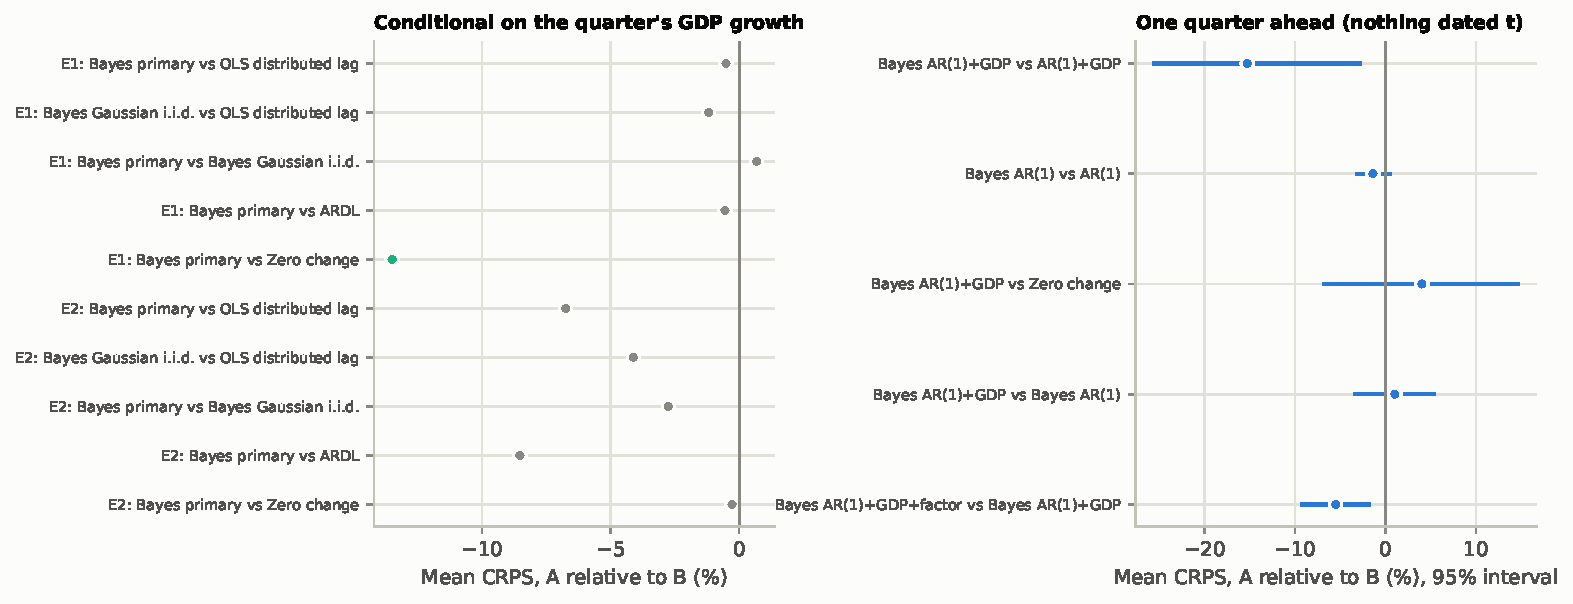
\includegraphics[width=\textwidth]{fig3_prediction.pdf}
\caption{Pre-registered predictive comparisons, mean CRPS of model A relative to model B
(negative: A better). Left: conditional on the quarter's GDP growth (green: decided at the
5\% familywise level). Right: one-quarter-ahead forecasts with 95\% bootstrap percentile
intervals. A percentile interval can exclude zero while the registered null-centred,
Holm-adjusted test does not reject, because two pandemic quarters skew the bootstrap
distribution.}\label{fig:prediction}
\end{figure}

\section{Structural identification and its limits}\label{sec:identification}

\subsection{The problem}

Let $x_{it}$ collect GDP growth, the unemployment change and related variables, with
reduced-form dynamics
\[
  x_{it}=c_i+\sum_{l=1}^{p}A_l x_{i,t-l}+u_{it},\qquad \E[u_{it}u_{it}']=\Sigma .
\]
A structural model posits $u_{it}=B\varepsilon_{it}$ with mutually uncorrelated shocks
$\varepsilon_{it}$, so $\Sigma=BB'$. For any orthonormal $Q$, $BQ$ fits the data equally
well, which leaves $n(n-1)/2$ free parameters that identifying information must supply.

\paragraph{Innovations are not shocks.} Reduced-form innovations, and impulse responses
orthogonalised by an arbitrary ordering, are not structural shocks. By
equation~\eqref{eq:weighted}, a causal Okun coefficient must refer to a specific identified
shock $k$: the ratio $\kappa_k$ of its effects on unemployment and on output.

\paragraph{Strategies evaluated.} Four strategies were considered before any estimate:
\begin{itemize}
  \item \emph{Recursive orderings:} rejected. GDP and unemployment respond within the
    quarter to every shock, so no zero restriction between them is credible.
  \item \emph{Long-run restrictions} \citep{blanchard1989quah}: rejected. They assume two
    shocks and long-run neutrality, are unreliable in short samples
    \citep{faust1997longrun}, and conflate productivity with labour supply.
  \item \emph{External instruments} \citep{stock2018external}: estimated.
  \item \emph{Sign restrictions} \citep{rubio2010svar}: estimated, with inference that
    does not depend on the prior over rotations.
\end{itemize}
Local projections \citep{jorda2005lp} are an estimator, not an identification strategy.
They estimate the same responses as VARs in population \citep{plagborg2021lpvar}.

\subsection{External instruments}

\paragraph{The shocks.} Two common shocks are identified outside this study, each by
high-frequency event windows:
\begin{itemize}
  \item ECB monetary policy surprises, purged of central-bank information effects by sign
    restrictions on interest rates and stock prices
    \citep{jarocinski2020information,altavilla2019mpd};
  \item OPEC oil supply news \citep{kanzig2021oil}.
\end{itemize}
Neither is a productivity shock. No credible instrument exists for productivity or
labour-supply shocks in EU countries.

\paragraph{The local projections.} For horizon $h$, lag-augmented local projections are
estimated, pooled over countries with country effects and clustered by quarter
\citep{montielolea2021lp}:
\[
  y_{i,t+h}-y_{i,t-1}=a_i^h+b^h s_t+\sum_{l=1}^{L}\big(c_l^h s_{t-l}+d_l^{h\prime} x_{i,t-l}\big)
  +e_{it}^h .
\]
The shock-conditional ratio $\kappa(h)$ of cumulative unemployment to cumulative output
responses is estimated by LP-IV. Its Anderson--Rubin set
\citep{anderson1949ar} remains valid however weak the instrument:
\[
  \Big\{\kappa:\ (\hat b_u-\kappa\hat b_y)^2\le c^2\,\widehat{\operatorname{Var}}
  (\hat b_u-\kappa\hat b_y)\Big\}.
\]
The set is bounded exactly when the first-stage $|t|$ exceeds the critical value $c$, so an
unbounded set means the data do not determine the ratio.

\paragraph{Timing.} The shocks are monthly and are summed within each quarter, so a shock
late in a quarter has little time to act before the quarter ends. Even so, a 10 basis
point monetary tightening comes with an unemployment rate \val{id_mp_u0} percentage points
higher in the same quarter (90\% interval \val{id_mp_u0_ci}). A response that fast is
implausible for a policy shock. It points to timing within the quarter, to aggregation, or
to news about the economy contained in the policy surprise, and it is a further reason to
read these local projections cautiously.

\paragraph{Quarterly results.}
\begin{itemize}
  \item The first stages are weak: $|t|$ is at most \val{id_max_t}, against the
    conventional threshold of $3.16$ ($F=10$).
  \item All \val{id_sets} primary Anderson--Rubin sets are unbounded
    (table~\ref{tab:identification}).
  \item The quarterly sum of the oil surprise is predictable from lagged EU data
    ($p=$ \val{id_pred_oil}), which casts doubt on its exogeneity at that frequency. The
    monetary shock is not predictable ($p=$ \val{id_pred_mp}).
\end{itemize}

\paragraph{Monthly results.} A registered amendment kept the shocks at their native monthly
frequency, with monthly unemployment and industrial production as outcomes. The ratio is
then per unit of industrial production, not GDP. The primary sample was restricted to the
\val{mo_n_direct} countries whose monthly unemployment is a direct survey estimate. That restriction
defines a new assumption, that a month's value contains no later months, which a pre-shock
placebo tests.
\begin{itemize}
  \item At native frequency the oil surprise is not predictable ($p=$
    \val{mo_pred_oil}).
  \item The first stages remain weak (largest $|t|$ \val{mo_max_t}).
  \item All \val{mo_unbounded} primary sets are unbounded.
\end{itemize}

\subsection{Country-specific GDP shocks}

Identifying the effect of a country's own GDP shock requires an instrument that moves that
country's GDP and affects its unemployment only through GDP. The most defensible public
candidate is a shift-share of foreign demand
\citep{goldsmith2020bartik,borusyak2022shiftshare,adao2019shiftshare}:
\[
  Z_{it}=\sum_p e_{ip}\,g_{pt},
\]
where $e_{ip}$ is the share of country $i$'s value added absorbed in partner $p$'s final
demand \citep{oecd2025tiva} and $g_{pt}$ is partner GDP growth.

\paragraph{Partner sets.} Distant, non-European partners are the only set whose exclusion
restriction is defensible. Near partners bring migration and commuting, and intra-EU
partners share the European cycle.

\paragraph{Feasibility rule.} A registered rule required the expected first-stage $t$,
after country and quarter effects, to reach $3.16$ before any estimate. It is
\val{ss_P1_t} for distant demand. Adding near partners raises it only to \val{ss_P2_t}, and
intra-EU partners to \val{ss_P3_t}, while making exclusion indefensible. The design was
therefore not estimated.

\subsection{Sign restrictions}

\paragraph{The model.} A pooled panel VAR in GDP growth, deflator inflation and the changes
in unemployment and participation set-identifies three shocks by impact signs, following
the logic of \citet{foroni2018laborsupply}:
\begin{itemize}
  \item demand: $g+$, $\pi+$, $\Delta u-$;
  \item technology: $g+$, $\pi-$, $\Delta u-$;
  \item labour supply: $\pi-$, $\Delta u+$, $\Delta p+$.
\end{itemize}
The restriction on unemployment under technology is debatable: in sticky-price models,
employment can fall after a productivity improvement \citep{gali1999technology}. A
registered robustness check drops it.

\paragraph{Inference.} The usual uniform prior over rotations shapes the reported responses
\citep{baumeister2015sign}. We therefore report the identified set for every posterior draw
of the reduced form, summarised by the robust Bayesian approach of
\citet{giacomini2021robust}.

\paragraph{Results.}
\begin{itemize}
  \item \emph{Plausibility.} Every posterior draw admits the impact restrictions
    (\val{sr_nonempty}). Imposed also one quarter later, they are admissible in only
    \val{sr_nonempty_h01} of draws, so the data contradict that variant.
  \item \emph{Demand against technology.} The demand and technology sets for the Okun
    ratio are \val{sr_sets}. Demand- and technology-driven ratios cannot be distinguished.
  \item \emph{Why the ratios are unbounded.} This outcome is close to guaranteed by the
    design. The signs restrict impact responses only, and the ratio divides by the
    cumulative GDP response, whose admissible set includes zero (at eight quarters, for
    demand, \val{sr_dem_gdp8_ci}). The result shows that these restrictions are
    uninformative about the ratio; it is not evidence about the ratio's size. Bounds on
    elasticities or narrative sign restrictions would be the next step.
  \item \emph{Labour supply against demand.} They differ at impact only because the
    signs impose it. By eight quarters both robust regions for the unemployment response
    include zero. The robust region for each shock's share of the forecast-error variance
    of the quarterly change in unemployment (the VAR variable, not the level) runs from
    \val{sr_dem_fevd_lo} to \val{sr_dem_fevd_hi} for demand and from \val{sr_ls_fevd_lo}
    to \val{sr_ls_fevd_hi} for labour supply.
  \item \emph{The uniform prior.} It gives sharp-looking ratios (demand \val{sr_dem_uniform},
    technology \val{sr_tech_uniform}), but the sharpness comes from the prior, not from the
    data (figure~\ref{fig:sign}).
  \item \emph{Recursive orderings.} Reported only as a measure of sensitivity, the
    \val{sr_n_orderings} orderings move the orthogonalised ``GDP shock'' ratio between \val{sr_order_min_h4}
    and \val{sr_order_max_h4} at four quarters, depending on whether GDP is ordered before
    unemployment. None of them is causal.
\end{itemize}

\subsection{Testable and untestable assumptions}

\paragraph{Testable.}
\begin{itemize}
  \item instrument relevance (first-stage strength);
  \item predictability of a shock from lagged data, a partial test of exogeneity;
  \item the timing of monthly series (placebo);
  \item the joint compatibility of sign restrictions with the reduced form (non-emptiness).
\end{itemize}

\paragraph{Not testable.}
\begin{itemize}
  \item event-window exogeneity;
  \item the purity of the monetary shock;
  \item the exclusion restriction of foreign demand;
  \item the sign restrictions themselves;
  \item linearity and homogeneity of responses.
\end{itemize}

\subsection{A post-hoc check of the pandemic window}

The registered rules drop an observation if any period of its variables lies in
2020--2021. The quarterly window starts at $t-4$, the monthly window at $t-12$ and the VAR
window at $t-2$. The change at the longest lag, however, is measured from the level one
period earlier, which can fall in 2021 while the observation is kept. After an external
review we widened every window by one period. This check was not registered, and the
registered results remain primary:
\begin{itemize}
  \item quarterly: the largest first-stage $|t|$ is \val{ws_q0_max_t} with the registered
    window and \val{ws_q1_max_t} with the widened one, and \val{ws_q1_unbounded} sets
    remain unbounded;
  \item monthly: \val{ws_m0_max_t} and \val{ws_m1_max_t}, with \val{ws_m1_unbounded} sets
    unbounded;
  \item sign restrictions: every draw remains admissible (\val{ws_sr_nonempty}), and the
    demand and technology Okun-ratio regions are \val{ws_sr_regions}.
\end{itemize}
No conclusion changes.

\subsection{What the identification study shows}

With the public data available for the \eu, the instruments and restrictions we could
defend are uninformative about a causal Okun coefficient. That is a statement about these
designs, not about the size of any causal effect. Every coefficient in this study
therefore remains a reduced-form association. More informative answers would need:
\begin{itemize}
  \item utilisation-adjusted quarterly productivity series;
  \item quasi-experimental variation in labour supply;
  \item country-specific policy shocks, such as narrative fiscal shocks;
  \item regional data;
  \item longer break-free samples.
\end{itemize}

% Generated by eu-okun publication. Do not edit.
\begin{table}[t]\centering\small
\caption{First-stage strength and Anderson--Rubin (Fieller) 90\% sets of the shock-conditional ratio of unemployment to output responses. Quarterly: output is GDP; monthly: industrial production. Shift-share: benchmark expected first-stage $t$ (no estimate). The conventional weak-instrument threshold is $|t|=3.16$. Two rays: the union of two unbounded half-lines.}
\label{tab:identification}
\begin{tabular}{lllrl}
\toprule
Design & Instrument & Horizon & First-stage $t$ & 90\% AR set \\
\midrule
Quarterly LP-IV & ECB monetary policy & 4 quarters & $-0.64$ & unbounded \\
Quarterly LP-IV & ECB monetary policy & 8 quarters & $+0.02$ & two rays \\
Quarterly LP-IV & OPEC oil supply news & 4 quarters & $+1.27$ & unbounded \\
Quarterly LP-IV & OPEC oil supply news & 8 quarters & $+0.70$ & unbounded \\
Monthly LP-IV & ECB monetary policy & 12 months & $-0.22$ & unbounded \\
Monthly LP-IV & ECB monetary policy & 24 months & $+0.34$ & unbounded \\
Monthly LP-IV & OPEC oil supply news & 12 months & $+1.21$ & unbounded \\
Monthly LP-IV & OPEC oil supply news & 24 months & $+0.75$ & unbounded \\
Shift-share & distant demand & --- & $0.19$ & not estimated \\
Shift-share & + near extra-EU & --- & $0.31$ & not estimated \\
Shift-share & intra-EU leave-one-out & --- & $0.66$ & not estimated \\
\bottomrule
\end{tabular}
\end{table}


\begin{figure}[t]\centering
\begin{minipage}{0.49\textwidth}\centering
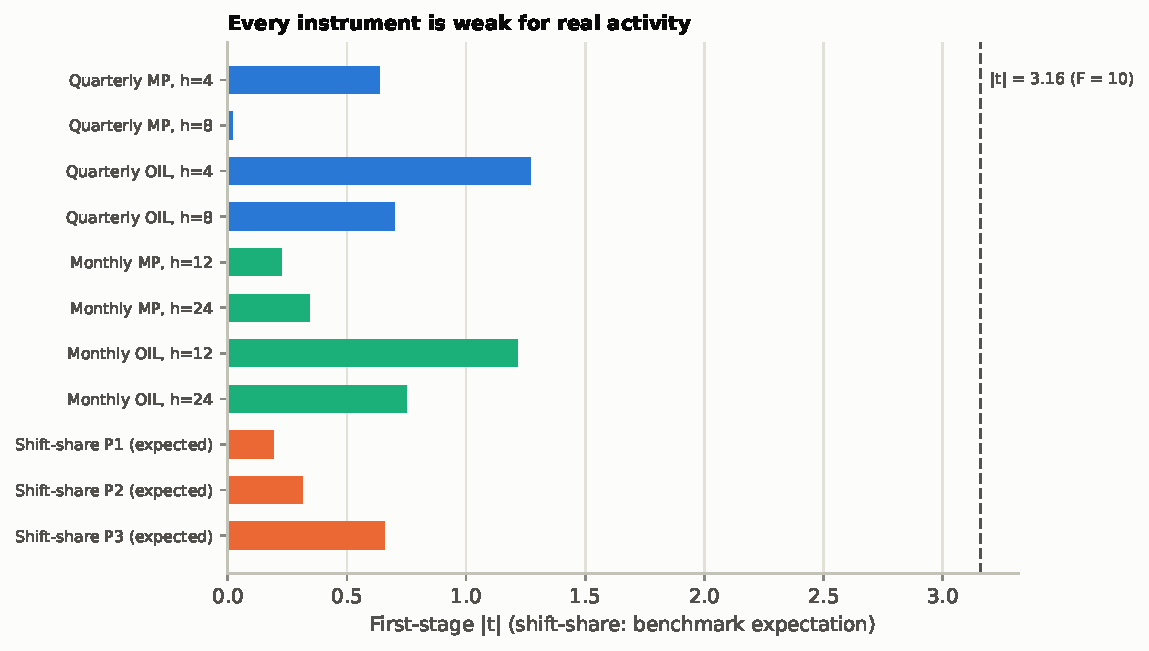
\includegraphics[width=\textwidth]{fig4_identification.pdf}
\end{minipage}\hfill
\begin{minipage}{0.49\textwidth}\centering
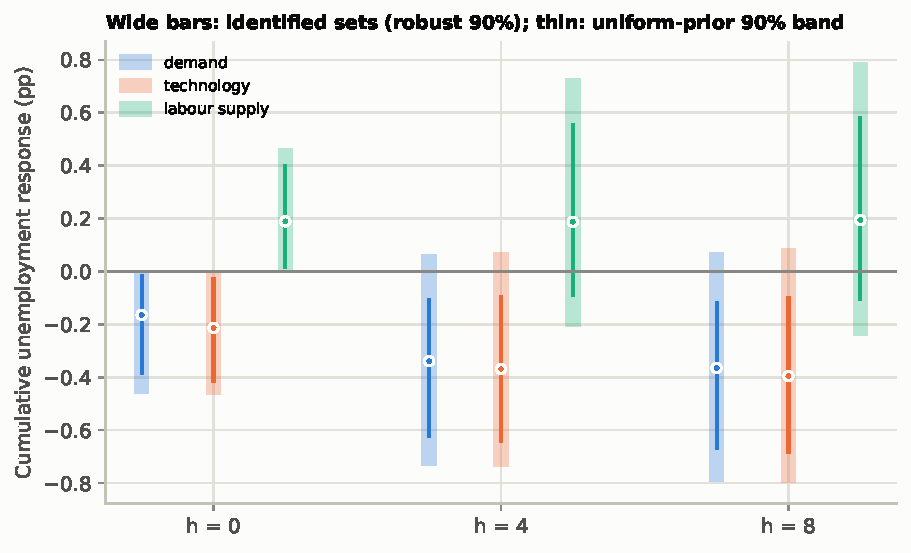
\includegraphics[width=\textwidth]{fig5_sign_restrictions.pdf}
\end{minipage}
\caption{Left: first-stage strength of every instrument (shift-share: benchmark
expectation); the dashed line is $|t|=3.16$. Right: cumulative unemployment responses to
one-standard-deviation shocks. Wide bars are robust 90\% regions of the identified sets;
thin lines and dots are the uniform-rotation posterior 90\% bands and medians.}
\label{fig:sign}
\end{figure}

\section{Portugal, Spain, the Netherlands and Luxembourg}\label{sec:cases}

\paragraph{Design.} The case study asks where output fluctuations are absorbed in four
countries. Each hypothesis was written down before any computation and follows from
definitions, from the accounting identity~\eqref{eq:identity} or from standard mechanisms.
Each makes predictions that can fail and that are evaluated by the same rule in the
comparison countries, so no prediction is tailored to one country. Three classes of
evidence are kept apart:
\begin{itemize}
  \item \emph{correlation}: cross-country associations with institutions;
  \item \emph{pattern consistent with a mechanism}: where output fluctuations are absorbed;
  \item \emph{identified causal effect}: none, because the designs of
    section~\ref{sec:identification} are uninformative.
\end{itemize}

\paragraph{Margins.} Each margin's response is the two-lag sum of its elasticity to GDP
growth, with 2020--2021 excluded. Intervals are 95\% synchronised circular block-bootstrap
intervals \citep{kunsch1989bootstrap}. By the identity, the elasticities of output per hour,
hours per worker and domestic employment sum to one.

\paragraph{Data.} The employment and hours data come from the national accounts
(\citetalias{eurostat_namq_10_pe}, \citetalias{eurostat_namq_10_a10_e}). Temporary and permanent employees
come from the Labour Force Survey (\citetalias{eurostat_lfsq_etgaed}, \citetalias{eurostat_lfsq_eegaed}), the
cross-country temporary and part-time shares from
\citetalias{eurostat_lfsq_etpga} and \citetalias{eurostat_lfsq_eppga}, and employment protection indicators from
the OECD \citep{oecd2020epl}. Eurostat publishes hours worked for Portugal but no
seasonally adjusted quarterly employment in persons, so its hours per worker and domestic
employment cannot be computed and two of its predictions cannot be evaluated. The protocol
had assumed wider coverage; its change log records the correction.

\paragraph{Overall result.} \val{cs_supported} of \val{cs_total} pre-registered predictions
is supported and \val{cs_contradicted} are contradicted; the rest are not determined
(table~\ref{tab:casestudy}). The cross-country correlations with institutions are a
separate, registered set of \val{cs_n_corr} correlations (subsection~\ref{sec:institutions}),
outside these \val{cs_total} predictions.

\subsection{Spain}

\paragraph{Association.} Spain's association is large and robust:
\begin{itemize}
  \item classical two-lag sum \val{cl_ES_excl} \val{cl_ES_excl_ci} for 2009--2026 without
    2020--2021;
  \item on the same 2009--2019 quarters, OLS gives \val{by_ES_ols} and the hierarchical
    model \val{by_ES} \val{by_ES_ci}; the gap is partly pooling and partly the common
    factor, which the hierarchical sum excludes;
  \item probability \val{claim_es_p} that its sum lies below the European mean, with the
    rule satisfied in \val{claim_es_holds} of \val{by_n_accepted} accepted fits.
\end{itemize}

\paragraph{Margins.} Spain absorbs output fluctuations almost entirely through
employment (figure~\ref{fig:margins}):
\begin{itemize}
  \item domestic-employment elasticity \val{cs_ES_e_dom} \val{cs_ES_e_dom_ci};
  \item output per hour \val{cs_ES_prod} \val{cs_ES_prod_ci}, an interval that includes
    zero.
\end{itemize}
\citet{bentolila2012twotier} attribute much of Spain's larger rise in unemployment in the
Great Recession, compared with France, to the gap between the dismissal costs of permanent
and temporary contracts. The pre-registered test that temporary employment is more
GDP-elastic than permanent employment gives \val{cs_p41es} \val{cs_p41es_ci} and is
\val{cs_p41es_verdict}. It is supported only in the \val{cs_p41es_settings} sensitivity
setting. The data therefore do not establish that temporary contracts carry Spain's
adjustment, and do not show that they cause it.

\subsection{Portugal}

\paragraph{Association.} Portugal's association is negative, but its significance depends
on the specification:
\begin{itemize}
  \item full sample: \val{cl_PT_full} \val{cl_PT_full_ci};
  \item without 2020--2021: \val{cl_PT_excl} \val{cl_PT_excl_ci};
  \item posterior median: \val{by_PT} \val{by_PT_ci}.
\end{itemize}
The Spain--Portugal difference \val{pair_ES_PT} the robustness set
(section~\ref{sec:heterogeneity}).

\paragraph{Margins.} Total hours respond to GDP almost as strongly in Portugal
(\val{cs_PT_h} \val{cs_PT_h_ci}) as in Spain (\val{cs_ES_h} \val{cs_ES_h_ci}). The
Spain--Portugal difference in the unemployment response \val{cs_pair_ES_PT_h} when
measured in hours worked.

\paragraph{Predictions.} The prediction that Portugal adjusts more through productivity
than Spain gives \val{cs_p52} \val{cs_p52_ci} and is \val{cs_p52_verdict}. The employment
comparison cannot be made with the published data.

\paragraph{A descriptive observation.} The following was not a registered prediction.
Participation rises with GDP in Portugal (\val{cs_PT_dp} \val{cs_PT_dp_ci} percentage
points per percent) but not in Spain. By identity~\eqref{eq:identity}, a labour force that
grows with output offsets part of the fall in unemployment that employment growth would
otherwise bring. With total hours responding alike in the two countries, this is one
accounting route to Portugal's smaller unemployment response. Whether it is the route
cannot be checked without quarterly employment in persons.

\subsection{The Netherlands}

\paragraph{Timing.} The posterior share of the Dutch response that comes from lagged GDP
growth is \val{by_NL_lagshare}. The registered rule for a delayed response holds in the
primary fit (probability \val{claim_nl_p}) but only in \val{claim_nl_holds} of
\val{by_n_accepted} accepted fits. Measured with four lags, the Dutch lagged share exceeds
Spain's by \val{cs_p31a} \val{cs_p31a_ci}, which is \val{cs_p31a_verdict} (supported only
in the \val{cs_p31a_settings} setting).

\paragraph{Margins.}
\begin{itemize}
  \item \emph{Output per hour:} the one supported prediction. Dutch output per hour is
    more GDP-elastic than Spanish, by \val{cs_p22} \val{cs_p22_ci} (Holm $p=$
    \val{cs_p22_holm}). A larger productivity response is a pattern consistent with labour
    hoarding, although hoarding cannot be separated from unmeasured effort or capacity
    utilisation.
  \item \emph{Hours per worker:} the difference from Spain, \val{cs_p21a} \val{cs_p21a_ci},
    is \val{cs_p21a_verdict}.
  \item \emph{Participation:} it responds less in the Netherlands than in Portugal
    (\val{cs_p23b} \val{cs_p23b_ci}, Holm $p=$ \val{cs_p23b_holm}), the opposite of the
    prediction, but this is not decided after adjustment.
\end{itemize}

\subsection{Luxembourg}

\paragraph{Association.}
\begin{itemize}
  \item \emph{Classical:} the sum is \val{cl_LU_verdict}: \val{cl_LU_full} on the full
    sample, \val{cl_LU_excl} without 2020--2021.
  \item \emph{Bayesian:} the posterior median is \val{by_LU} \val{by_LU_ci}.
  \item \emph{The weakness rule} requires the sum to lie above the European mean with
    probability at least $0.95$ and its 90\% interval to include zero. That probability is
    \val{claim_lu_p} in the primary fit, and the rule holds in \val{claim_lu_holds} of
    \val{by_n_accepted} accepted fits.
  \item \emph{The dynamic amendment.} In the two ARDL fits, which model the persistence
    the primary model misses, the rule \val{dyn_lu_ardl} on the long-run sum
    (probabilities \val{dyn_lu_ardl_p} and \val{dyn_lu_adf_p}). It holds because of
    Luxembourg's negative lagged-change coefficient, which shrinks its long-run multiplier;
    on the short-run sum the probability is \val{dyn_lu_adf_short_p}. These fits were
    registered as an amendment and are not part of the claim judgement, which keeps the
    original nine specifications.
\end{itemize}

\paragraph{Measurement.} GDP counts production by everyone working in Luxembourg, while
unemployment counts residents only, and cross-border commuters are a large share of
employment. If labour-input adjustment fell on commuters, domestic employment would respond
more than resident employment. It does not: the gap is \val{cs_p11} \val{cs_p11_ci}, and
both measures barely move with GDP:
\begin{itemize}
  \item domestic employment: \val{cs_LU_e_dom_pe} \val{cs_LU_e_dom_pe_ci};
  \item resident employment: \val{cs_LU_e_res} \val{cs_LU_e_res_ci}.
\end{itemize}
Instead, measured output per hour moves almost one for one with measured GDP
(\val{cs_LU_prod} \val{cs_LU_prod_ci}).

\paragraph{Two rival explanations, tested.} Output per hour is computed as the residual
$g-h$, where $h$ is the growth of hours. A weak link between output and labour input can
therefore come from the data as well as from the economy. A further registered study
(\texttt{GDP\_MEASUREMENT\_PROTOCOL.md}) tested two explanations with value added and
hours by industry \citepalias{eurostat_namq_10_a10}. Each test compares Luxembourg with
the median of the countries outside Luxembourg, Ireland and Malta.
\begin{itemize}
  \item \emph{Transitory noise in quarterly output.} If quarterly growth carried noise
    unrelated to labour input, measured growth would be negatively autocorrelated, and the
    correlation of hours with output would rise more than elsewhere once both are measured
    year on year, because aggregation averages the noise out. Luxembourg's growth
    autocorrelation is lower than the comparison group's (\val{gm_p11_lu_focus} against
    \val{gm_p11_lu_median}; Holm $p=$ \val{gm_p11_lu_holm}, \val{gm_p11_lu_verdict}). But
    its hours-output correlation does not rise at all: it is \val{gm_lu_c_q} quarter on
    quarter and \val{gm_lu_c_y} year on year, while it rises by a median
    \val{gm_p12_lu_median} elsewhere. That points away from noise, although it is not
    decided after adjustment (difference \val{gm_p12_lu} \val{gm_p12_lu_ci}, Holm
    $p=$ \val{gm_p12_lu_holm}).
  \item \emph{The financial sector.} Finance is \val{gm_lu_fin_va} of Luxembourg's value
    added and \val{gm_lu_fin_hours} of its hours; the next highest share of value added is
    about \val{gm_fin_va_next}. Yet removing finance from both output and hours barely
    changes the link. The hours elasticity changes by \val{gm_p21_lu_focus} and the Okun
    sum by \val{gm_p22_lu_focus} (verdicts: \val{gm_p21_lu_verdict} and
    \val{gm_p22_lu_verdict}).
    The output-per-hour elasticity is \val{gm_lu_prod} for all industries and
    \val{gm_lu_prod_n} outside finance.
\end{itemize}
By the interpretation rules fixed in that protocol, both explanations fail their tests,
and Luxembourg's weak output-labour link remains unexplained. Of
\val{gm_total} predictions, \val{gm_supported} is supported: Ireland's quarterly growth
is negatively autocorrelated (\val{gm_p11_ie_focus} against \val{gm_p11_ie_median}),
the signature of noise in its quarterly output. Its year-on-year correlation rises like
everyone else's, however, so the full signature is not established there either.
Ireland's modified domestic demand, published by its statistical office rather than
Eurostat, and sectoral composition beyond finance were not tested.

\subsection{Do the differences remain under other measures?}

\paragraph{Test.} If a difference between two countries reflects how much of their
labour-input adjustment falls on unemployment, it may disappear when labour input is
measured by employment or hours. Each pair whose unemployment responses differ was compared
again under resident employment, domestic employment and hours worked, where the data
exist. Of these pair-and-measure comparisons:
\begin{itemize}
  \item \val{cs_pairs_remain} remain;
  \item \val{cs_pairs_disappear} disappear;
  \item \val{cs_pairs_reverse} reverse.
\end{itemize}

\paragraph{By pair, in hours worked.}
\begin{itemize}
  \item Spain--Netherlands: \val{cs_pair_ES_NL_h};
  \item Spain--Luxembourg: \val{cs_pair_ES_LU_h};
  \item Spain--Portugal: \val{cs_pair_ES_PT_h};
  \item Netherlands--Luxembourg: \val{cs_pair_NL_LU_h}.
\end{itemize}

\subsection{Institutions}\label{sec:institutions}

The protocol predicted that stricter employment protection would weaken the unemployment
response. Spearman correlations across countries were computed with permutation $p$-values,
Holm-adjusted over six indicators in each of three variants. Of the \val{cs_n_corr}
correlations, \val{cs_n_corr_contra} point the other way at the registered level:
\begin{itemize}
  \item regular-contract protection against the classical sum: $\rho=$
    \val{cs_eplr_cl_rho} over \val{cs_eplr_cl_n} countries (Holm $p=$
    \val{cs_eplr_cl_holm});
  \item temporary-contract protection against the Bayesian sum without Luxembourg and
    Ireland: $\rho=$ \val{cs_eplt_noluie_rho} over \val{cs_eplt_noluie_n} countries (Holm
    $p=$ \val{cs_eplt_noluie_holm}).
\end{itemize}
With all twenty countries the second correlation is \val{cs_eplt_by_rho} (Holm $p=$
\val{cs_eplt_by_holm}). These are correlations among at most twenty countries, measured
once in 2008. They contradict the predicted direction, but they say nothing about what
employment protection does.

\subsection{Comparison with the earlier claims}

Table~\ref{tab:claims} sets the earlier analysis's three descriptive claims, and the two
explanations we tested of the kind it suggested, against the evidence. No claim about Portugal was documented, so none
is assessed. Several explanations could not be
tested reliably, and the protocol said so before any result:
\begin{itemize}
  \item the 2012 labour-market reforms in Spain and Portugal, which coincide with the
    sovereign-debt crisis;
  \item short-time work, for which no harmonised quarterly take-up data exist before 2020;
  \item collective bargaining, minimum wages and benefit generosity;
  \item sectoral composition.
\end{itemize}

\begin{table}[t]\centering\small
\caption{The earlier claims against the evidence. ``Supported'': the evidence agrees under
every accepted specification. ``Qualified'': part of the claim holds, or it holds only
under some specifications. ``Contradicted'': the evidence points the other way at the
registered level. None of these verdicts is causal.}\label{tab:claims}
\begin{tabular}{p{0.2\textwidth}p{0.5\textwidth}p{0.2\textwidth}}
\toprule
Claim & Evidence & Verdict \\
\midrule
Spain: large association
  & Below the European mean with probability \val{claim_es_p}; rule holds in
    \val{claim_es_holds} of \val{by_n_accepted} accepted fits. Adjustment runs through
    employment (\val{cs_ES_e_dom}).
  & Supported \\
\addlinespace
Netherlands: delayed response
  & Lag share \val{by_NL_lagshare}; rule holds in \val{claim_nl_holds} of
    \val{by_n_accepted} fits. Lag share against Spain \val{cs_p31a_verdict}. Output per hour
    absorbs more than in Spain (Holm $p=$ \val{cs_p22_holm}).
  & Qualified \\
\addlinespace
Luxembourg: weak association
  & Classical sum \val{cl_LU_verdict}; Bayesian rule holds in \val{claim_lu_holds} of
    \val{by_n_accepted} registered fits, but \val{dyn_lu_adf} on the long-run sum in both
    ARDL amendment fits.
  & Qualified \\
\addlinespace
Explanation: the commuter mismatch
  & Domestic-minus-resident gap \val{cs_p11} \val{cs_p11_ci}. The two rival explanations
    tested afterwards, transitory noise in quarterly output and the financial sector, fail
    their tests too.
  & Not supported \\
\addlinespace
Explanation: employment protection weakens the response
  & \val{cs_n_corr_contra} of \val{cs_n_corr} registered correlations have the opposite
    sign at the registered level (\val{cs_eplr_cl_rho}, \val{cs_eplt_noluie_rho}); the
    rest are not determined.
  & Contradicted (correlation only) \\
\bottomrule
\end{tabular}
\end{table}

% Generated by eu-okun publication. Do not edit.
\begin{table}[t]\centering\small
\caption{Pre-registered predictions of the case study (two-lag elasticities to GDP growth, 2020--2021 excluded; block-bootstrap 95\% intervals; Holm adjustment over the determinable predictions). A supported prediction is a pattern consistent with a mechanism, not a causal effect.}
\label{tab:casestudy}
\footnotesize
\begin{tabular}{llrrl}
\toprule
Prediction & Statistic & Estimate [95\%] & Holm $p$ & Verdict \\
\midrule
P1.1 & \texttt{beta\_e\_dom\_pe(LU) - beta\_e\_res(LU)} & $+0.01$ $[-0.05, +0.05]$ & $1.000$ & not determined \\
P1.3 & \texttt{gap(LU) - median gap(others)} & $+0.00$ $[-0.06, +0.05]$ & $1.000$ & not determined \\
P2.1a & \texttt{beta\_hpw(NL) - beta\_hpw(ES)} & $-0.08$ $[-0.60, +0.23]$ & $1.000$ & not determined \\
P2.1b & \texttt{beta\_hpw(NL) - beta\_hpw(PT)} & n/a & n/a & not determined \\
P2.2 & \texttt{beta\_prod(NL) - beta\_prod(ES)} & $+0.73$ $[+0.31, +1.23]$ & $0.022$ & supported \\
P2.3a & \texttt{beta\_dp(NL) - beta\_dp(ES)} & $-0.01$ $[-0.15, +0.15]$ & $1.000$ & not determined \\
P2.3b & \texttt{beta\_dp(NL) - beta\_dp(PT)} & $-0.22$ $[-0.39, -0.06]$ & $0.100$ & not determined \\
P3.1a & \texttt{share(NL) - share(ES)} & $+0.46$ $[-0.13, +1.04]$ & $1.000$ & not determined \\
P3.1b & \texttt{share(NL) - share(PT)} & n/a & n/a & not determined \\
P4.1 ES & \texttt{beta\_temp(ES) - beta\_perm(ES)} & $+0.72$ $[-1.28, +2.08]$ & $1.000$ & not determined \\
P4.1 PT & \texttt{beta\_temp(PT) - beta\_perm(PT)} & $+0.10$ $[-1.51, +1.16]$ & $1.000$ & not determined \\
P4.1 NL & \texttt{beta\_temp(NL) - beta\_perm(NL)} & $-0.46$ $[-2.07, +1.06]$ & $1.000$ & not determined \\
P5.1 & \texttt{beta\_e\_dom(ES) - beta\_e\_dom(PT)} & n/a & n/a & not determined \\
P5.2 & \texttt{beta\_prod(PT) - beta\_prod(ES)} & $-0.06$ $[-0.51, +0.28]$ & $1.000$ & not determined \\
\bottomrule
\end{tabular}
\end{table}


\begin{figure}[t]\centering
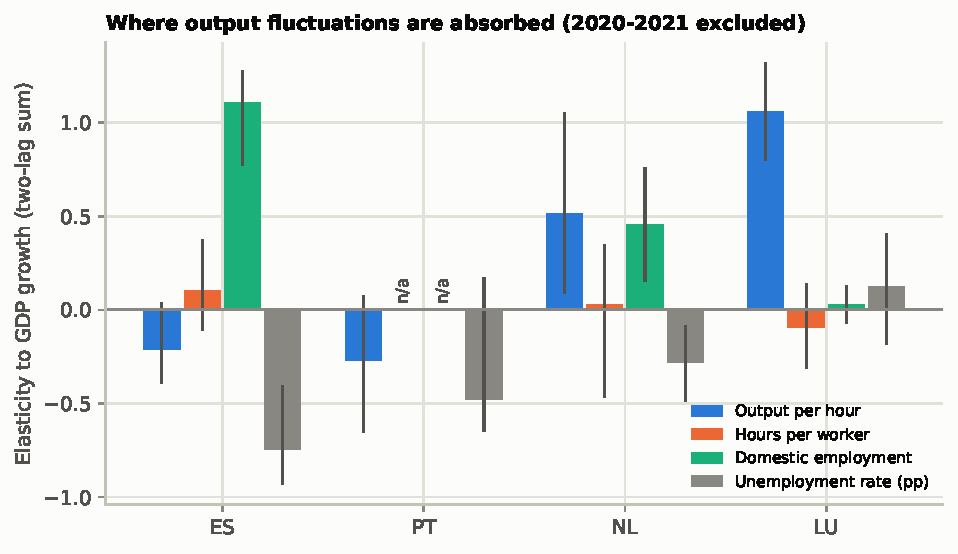
\includegraphics[width=0.8\textwidth]{fig6_margins.pdf}
\caption{Elasticities to GDP growth of output per hour, hours per worker, domestic
employment and the unemployment rate (two-lag sums, 2020--2021 excluded, 95\%
block-bootstrap intervals). Eurostat publishes no seasonally adjusted quarterly employment
in persons for Portugal, so its hours per worker and domestic employment are not
available. Portugal's unemployment elasticity, \val{cs_PT_du} \val{cs_PT_du_ci}, has a
bootstrap interval that crosses zero, while the HAC interval of table~\ref{tab:countries}
(\val{cl_PT_excl} \val{cl_PT_excl_ci}) does not. The point estimates agree; the
percentile interval of the block bootstrap is wide and asymmetric, which suggests a few
influential quarters, whereas the HAC interval relies on normal critical
values.}\label{fig:margins}
\end{figure}

\section{Discussion}\label{sec:discussion}

\subsection{Association, prediction and causation}

\paragraph{Association.} The three questions of the introduction have different answers.
The association is established: outside 2020--2021, faster GDP growth goes with a falling
unemployment rate in nearly every member state. Its size is not a single number:
\begin{itemize}
  \item it depends on whether the pandemic quarters are included;
  \item it depends on whether the error model absorbs residual persistence and a common
    European factor;
  \item the hierarchical sum is smaller than the classical one in \val{by_n_smaller} of
    \val{n_countries} countries, partly because the two estimate different quantities.
\end{itemize}

\paragraph{Prediction.} The association predicts little that the recent path of
unemployment does not already contain. The one decided comparison involves the quarter's
own GDP growth, which a forecaster would not know.

\paragraph{Causation.} No strategy available with public data identifies a causal Okun
coefficient for any shock. The coefficients reported here should be read as conditional
associations: summaries of how unemployment and output moved together in a period with a
particular mix of shocks.

\subsection{Positive, negative and unstable results}

\paragraph{Positive.} Results that the registered tests decide:
\begin{itemize}
  \item a negative association in \val{cl_n_neg_excluded} of \val{n_countries} countries
    without 2020--2021, robust to the core specifications in \val{cl_n_robust};
  \item \val{by_n_neg_all} sums credibly negative in every accepted Bayesian fit;
  \item Spain's large association, relative to the European mean;
  \item the Spain--Luxembourg and Spain--Netherlands differences, which survive every
    accepted fit and remain when labour input is measured by employment or hours;
  \item a more GDP-elastic output per hour in the Netherlands than in Spain, supported in
    the primary design and in the \val{cs_p22_settings} sensitivity settings;
  \item the conditional predictive gain over zero change before the pandemic
    (\val{pc_e1_zero}).
\end{itemize}

\paragraph{Negative.} Results where the registered test found nothing:
\begin{itemize}
  \item no decided gain from hierarchical pooling, GDP lags or the common factor in
    one-quarter-ahead forecasts;
  \item none of the \val{ss_published_holm} published post-2021 changes survives
    small-sample inference;
  \item no informative causal coefficient from external instruments, shift-share or sign
    restrictions;
  \item no sign that Luxembourg's commuters absorb its output fluctuations;
  \item \val{cs_supported} of \val{cs_total} case-study predictions supported.
\end{itemize}

\paragraph{Unstable.} Results that depend on choices or runs:
\begin{itemize}
  \item the magnitude of the association, through the pandemic quarters and the error
    model;
  \item \val{by_pairs_primary} credible country differences in the primary fit against
    \val{by_pairs_surviving} in every accepted fit;
  \item the Dutch delayed response, which holds in \val{claim_nl_holds} of
    \val{by_n_accepted} accepted fits;
  \item Portugal's significance across samples;
  \item two case-study predictions supported only before 2020;
  \item the employment-protection correlations, each decided in one of three variants;
  \item the acceptance of two Bayesian sensitivity fits, which differed between the
    Windows run and its Linux replication. The claim verdicts were identical under both
    acceptance sets, and the report states the robustness judgements under each.
\end{itemize}

\subsection{Limitations}

\paragraph{Data.}
\begin{itemize}
  \item All data are revised vintages, so the forecasts are retrospective.
  \item The Labour Force Survey's 2021 redesign introduces flagged and unflagged
    discontinuities. The Bayesian models mask the flagged observations, but the Dutch
    phase-in is not flagged.
  \item Monthly unemployment is a direct estimate in only eight countries.
  \item Hours per worker and employment in persons are unavailable for seven countries,
    including Portugal.
\end{itemize}

\paragraph{Models.}
\begin{itemize}
  \item The primary Bayesian model understates the persistence of unemployment changes.
    The registered amendment that removes this misfit has a common factor correlated with
    average GDP growth (\val{dyn_factor_corr}), so its country sums measure the association
    beyond part of the common GDP cycle.
  \item The post-2021 sample has about seventeen quarters. It is too short to test a
    change in the association with useful power.
  \item Country-level correlations with institutions use at most twenty countries and a
    single year of indicators.
\end{itemize}

\subsection{Open questions}

The study leaves these questions unresolved:
\begin{enumerate}
  \item Do countries differ because their labour markets respond differently to the same
    shock, or because they face different mixes of shocks?
    Equation~\eqref{eq:weighted} shows that both produce different Okun coefficients;
    separating them requires shock-specific identification.
  \item What is the effect on unemployment of a productivity or labour-supply shock in an
    EU country? This needs utilisation-adjusted productivity and quasi-experimental
    variation in labour supply.
  \item Why does output per hour absorb almost all output fluctuations in Luxembourg?
  \item Do temporary contracts carry Spain's employment adjustment? The direction is
    consistent with that view, but the registered test is not decided.
  \item Did the association weaken after 2021? This can only be answered with a longer
    sample.
\end{enumerate}

\section{Conclusions}\label{sec:conclusions}

\paragraph{Association.} In the \eu\ from 2009 to 2026, the negative association between
quarterly GDP growth and the change in the unemployment rate is a robust descriptive
regularity outside the pandemic quarters. A hierarchical model that accounts for
heavy-tailed errors, residual persistence and a common European factor puts the average
country sum at \val{by_mu}, with a between-country standard deviation of \val{by_tau}.

\paragraph{Heterogeneity.} Some country differences are credible in every accepted
specification and persist under other measures of labour input; Spain against the
Netherlands and against Luxembourg are the clearest cases. Most rankings are not
established.

\paragraph{Prediction.} The association adds little to forecasts of unemployment, and
partial pooling does not improve them by more than sampling variation.

\paragraph{Causation.} No identification strategy available with public data turns the
association into a causal effect.

\paragraph{The earlier claims.} Spain's large association is supported. The other two are
qualified. The Dutch delayed response meets its registered rule in the primary fit but not
in every accepted specification. Luxembourg's association is weak and sign-unstable in the
classical estimates, but the registered Bayesian rule for a weak association is met in
none of the accepted fits. The proposed explanation for Luxembourg, the mismatch
between production by cross-border commuters and resident unemployment, is not supported:
domestic and resident employment barely move with GDP, and output per hour absorbs the
fluctuations.

\paragraph{The general lesson.} An Okun coefficient estimated from aggregate data is a
summary of how output and unemployment moved together over a particular period. It is not
a structural parameter of a country's labour market.


\bibliographystyle{plainnat}
\bibliography{references}

\appendix
\section{Reproducibility}\label{app:repro}

\paragraph{Repository.} All code, frozen data, protocols, result tables and this
manuscript are in the public repository \texttt{DiogoRibeiro7/Medium-Blog}, directory
\texttt{eu-okun-law}. The file \texttt{publication/README.md} gives the reproduction
steps command by command.

\paragraph{Data.} Every input is a frozen snapshot (table~\ref{tab:snapshots}):
\begin{itemize}
  \item the raw API responses, stored byte for byte;
  \item a manifest with the SHA-256 of every file, the request URL and the download time;
  \item a derived panel.
\end{itemize}
An audit re-derives each panel from the raw responses and compares hashes. The quarterly
panel's manifest begins \val{hash_quarterly}; \texttt{publication/manifest/data.json} lists
every file of every snapshot with its hash.

\paragraph{Analyses.} Each analysis has a protocol, a command that regenerates its
committed outputs from the snapshots, fixed seeds and an independent replication
(table~\ref{tab:experiments}). The Bayesian analyses were run on Windows 11 and replicated
on Ubuntu by GitHub Actions; posterior medians agree within the tolerances stated in each
report. MCMC draws are not bit-identical across platforms. Tables, figures and the values
quoted in the text are therefore built from the committed outputs, not from fresh draws.

\paragraph{Environment.} The environment is locked by Poetry (table~\ref{tab:environment}).
CI installs it with \texttt{poetry install} from the lock file and checks the lock with
\verb|poetry check --lock|.

\paragraph{From results to manuscript.} One function reads every number quoted in this
article from the committed result tables and records the source file of each. It writes
two outputs from the same values:
\begin{itemize}
  \item the LaTeX macros behind every \verb|\val{key}| in the text, and an error stops
    compilation if a key is undefined;
  \item the placeholders of the Medium version.
\end{itemize}
Tables~\ref{tab:countries}, \ref{tab:predictive}, \ref{tab:identification},
\ref{tab:casestudy} and the tables of this appendix and the next are generated by code, as
are all figures. Table~\ref{tab:data} and table~\ref{tab:claims} are written by hand: the
first describes sources, and every number in the second is a \verb|\val| macro.

\paragraph{The audit.} Before the build, an audit checks four things:
\begin{itemize}
  \item every snapshot against its manifest;
  \item consistency across outputs: Bayesian country medians against the robustness
    tables, the OLS column against a re-fit on the same rows, and claim verdicts and
    counts against the reports that state them;
  \item the numbers quoted in the README, the identification study and the roadmap,
    against the result tables;
  \item the bibliography. Every DOI is resolved at \texttt{doi.org}, and the registered
    title is compared with the entry; for Eurostat datasets, whose registered titles are
    not in English, the dataset code is compared instead. Entries without a DOI have their
    URL checked. Two have neither a DOI nor a URL: a book identified by its ISBN and
    \citet{okun1962}.
\end{itemize}
The results are in \texttt{publication/AUDIT.md} and
\texttt{publication/manifest/bibliography.json}.

\paragraph{Commands.} From \texttt{eu-okun-law}:
\begin{verbatim}
poetry install --extras dev
poetry run eu-okun publication --check
poetry run eu-okun publication --build
cd publication/manuscript
latexmk -pdf main.tex
\end{verbatim}
The commands that regenerate each analysis from the snapshots are listed in two places:
\texttt{publication/README.md} and \texttt{publication/manifest/experiments.json}.
The \verb|--check| step regenerates every text output in memory and fails if any
committed file differs. The workflow \texttt{eu-okun-law-estimates} runs it, the
publication tests and the \LaTeX\ build on every pull request that changes the project.

% Generated by eu-okun publication. Do not edit.
\begin{table}[htbp]\centering\small
\caption{Frozen snapshots: files and the first 16 hexadecimal digits of the SHA-256 of each snapshot's own manifest. Full per-file hashes are in \texttt{publication/manifest/data.json}.}
\label{tab:snapshots}
\begin{tabular}{lrl}
\toprule
Snapshot & Files & Manifest SHA-256 \\
\midrule
\texttt{ci-results-38754743850} & 8 & \texttt{09c0960894727682} \\
\texttt{eu-aggregate-2026-10-21} & 6 & \texttt{a5ccb971a68a20e3} \\
\texttt{eurostat-2026-10-15} & 6 & \texttt{8a8c8a107d584ba9} \\
\texttt{eurostat-2026-10-22} & 6 & \texttt{58feb8e65a3aee37} \\
\texttt{eurostat-deflator-2026-10-18} & 4 & \texttt{30900e56883b8a6e} \\
\texttt{eurostat-monthly-2026-10-18} & 5 & \texttt{ec2e65b6cbe8831f} \\
\texttt{external-shocks-2026-10-16} & 5 & \texttt{8361c685c67770e2} \\
\texttt{gdp-measurement-2026-10-19} & 9 & \texttt{7cc75f218c9e190d} \\
\texttt{heterogeneity-2026-10-18} & 13 & \texttt{4a6a6d1c82af1e3c} \\
\texttt{shift-share-2026-10-18} & 8 & \texttt{c5c914bb910b1e29} \\
\bottomrule
\end{tabular}
\end{table}

\begin{table}[htbp]\centering\small
\caption{Analyses: protocol, seeds and independent replication. The last rows are post-hoc checks added after external reviews, with no protocol. Commands and output fingerprints are in \texttt{publication/manifest/experiments.json}.}
\label{tab:experiments}
\scriptsize
\begin{tabular}{>{\raggedright\arraybackslash}p{0.3\textwidth}>{\raggedright\arraybackslash}p{0.25\textwidth}>{\raggedright\arraybackslash}p{0.11\textwidth}>{\raggedright\arraybackslash}p{0.22\textwidth}}
\toprule
Analysis & Protocol & Seeds & Replication \\
\midrule
Classical OLS/HAC estimates and their review & \texttt{METHODS.md} & 20261015 & 17 independent checks; outputs of CI run 38754743850, frozen in snapshots/\allowbreak{}ci-results-38754743850, reproduced \\
Small-sample inference for the post-2021 tests & \texttt{SMALL\_\allowbreak{}SAMPLE\_\allowbreak{}PROTOCOL.md} & 20261017, 20261018, 20261019 & regenerated by the offline test suite \\
Small-sample inference for the classical headline sums & \texttt{HEADLINE\_\allowbreak{}INFERENCE\_\allowbreak{}PROTOCOL.md} & 20261022, 20261023, 20261024 & regenerated by the offline test suite \\
The core robustness grid without the participation control & \texttt{CORE\_\allowbreak{}GRID\_\allowbreak{}PROTOCOL.md} & none & regenerated by the offline test suite \\
Does the quarterly unemployment rate inherit monthly smoothing? & \texttt{SMOOTHING\_\allowbreak{}PROTOCOL.md} & none & regenerated by the offline test suite \\
Measurement noise or finance? Luxembourg's weak output-labour link & \texttt{GDP\_\allowbreak{}MEASUREMENT\_\allowbreak{}PROTOCOL.md} & 20261025 & regenerated by the offline test suite \\
Okun's law in hours, for every country, with and without the pandemic & \texttt{HOURS\_\allowbreak{}PROTOCOL.md} & 20261026 & regenerated by the offline test suite \\
Asymmetry between expansions and contractions & \texttt{ASYMMETRY\_\allowbreak{}PROTOCOL.md} & 20261027 & regenerated by the offline test suite \\
A common-correlated-effects mean-group panel & \texttt{CCE\_\allowbreak{}PROTOCOL.md} & 20261028 & regenerated by the offline test suite \\
The EU as a whole: a labour-force-weighted aggregate & \texttt{AGGREGATE\_\allowbreak{}PROTOCOL.md} & 20261029 & regenerated by the offline test suite \\
Definition breaks and data vintages & \texttt{MEASUREMENT\_\allowbreak{}PROTOCOL.md} & 20261022, 20261023 & regenerated by the offline test suite \\
Hierarchical Bayesian estimates, checks, robustness, dynamics and regimes & \texttt{BAYES\_\allowbreak{}PROTOCOL.md} & 20261016 & Linux replications committed under each docs/\allowbreak{}bayes*/\allowbreak{}replication-linux \\
Diagnostics of the reported Bayesian results & \texttt{BAYES\_\allowbreak{}DIAGNOSTICS\_\allowbreak{}PROTOCOL.md} & 20261016, 20261018, 20261030, 20261031, 20261032, 20261033 & four further seeds; the report regenerates from its committed summary in the offline test suite \\
Conditional predictive comparison & \texttt{PREDICTIVE\_\allowbreak{}PROTOCOL.md} & 20261016 & GitHub Actions run 38879823246 (docs/\allowbreak{}predictive/\allowbreak{}replication-linux) \\
One-quarter-ahead forecasts, Bayesian against classical & \texttt{BAYES\_\allowbreak{}FORECAST\_\allowbreak{}PROTOCOL.md} & 20261016, 20261020 & GitHub Actions run 38919566372 (docs/\allowbreak{}forecast-comparison/\allowbreak{}replication-linux) \\
Local projections on externally identified shocks & \texttt{IDENTIFICATION\_\allowbreak{}PROTOCOL.md} & none & regenerated by the offline test suite \\
Monthly outcomes for the identified shocks & \texttt{MONTHLY\_\allowbreak{}IDENTIFICATION\_\allowbreak{}PROTOCOL.md} & none & GitHub Actions run 39116120661 \\
Feasibility of a foreign-demand shift-share instrument & \texttt{SHIFT\_\allowbreak{}SHARE\_\allowbreak{}PROTOCOL.md} & none & GitHub Actions run 39118428267 \\
Sign-restricted SVAR with robust Bayesian sets & \texttt{SIGN\_\allowbreak{}RESTRICTIONS\_\allowbreak{}PROTOCOL.md} & 20261018 & GitHub Actions run 39124106363 (job sign-restrictions) \\
Case study of Portugal, Spain, the Netherlands and Luxembourg & \texttt{HETEROGENEITY\_\allowbreak{}PROTOCOL.md} & 20261018 & GitHub Actions run 39129218012 \\
\midrule
The pandemic window widened by one period & not registered & 20261018 & regenerated by the offline test suite \\
Null-imposed bootstraps with errors from the unrestricted residuals & not registered & 20261017, 20261018, 20261022, 20261024 & regenerated by the offline test suite \\
\bottomrule
\end{tabular}
\end{table}

\begin{table}[htbp]\centering\small
\caption{Software environment, locked by \texttt{poetry.lock}.}
\label{tab:environment}
\begin{tabular}{ll}
\toprule
Component & Version \\
\midrule
Python & $\geq$3.12, $<$3.15 \\
Poetry & 2.5.1 (CI) \\
\texttt{arviz} & 1.3.0 \\
\texttt{h5netcdf} & 1.8.1 \\
\texttt{jax} & 0.11.2 \\
\texttt{jaxlib} & 0.11.2 \\
\texttt{matplotlib} & 3.11.2 \\
\texttt{numpy} & 2.5.4 \\
\texttt{numpyro} & 0.22.0 \\
\texttt{openpyxl} & 3.1.5 \\
\texttt{scipy} & 1.18.1 \\
\texttt{poetry.lock} SHA-256 & \texttt{4417bcf47e79d3f9} \\
\bottomrule
\end{tabular}
\end{table}


\section{Pre-registration record}\label{app:prereg}

\paragraph{Rule.} Each analysis was registered before it was run. Before any estimate, its
protocol was committed and pushed. The protocol fixes:
\begin{itemize}
  \item the data and sample;
  \item the estimator and its settings;
  \item the decision rules and multiple-comparison families;
  \item the sensitivity analyses;
  \item for the case study, the hypotheses that cannot be tested reliably.
\end{itemize}
Table~\ref{tab:prereg} lists the commit that first added each protocol. In every case the
commit precedes, in the repository history, the commit that first added the results.

\paragraph{Changes after registration.} A change made after registration is recorded in
the protocol's change log, with its timing relative to the results and its reason. Three
kinds of change occurred:
\begin{itemize}
  \item \emph{clarifications made before any estimate}: for example, the Bayesian claim
    rules when a specification has no population mean, and the treatment of an indicator
    without variation;
  \item \emph{corrections after the first computation that change no rule}: for example,
    the coverage of employment in persons;
  \item \emph{amendments}: registered extensions with their own decision rules, written
    before their fits. Examples are the dynamic and regime Bayesian models and the monthly
    identification.
\end{itemize}
Analyses added after results were seen, such as the checks of the common factor, are
labelled as exploratory in the protocol and in the report.

\paragraph{The classical plan.} \texttt{METHODS.md} is the research plan of the classical
stage. It was committed with the data pipeline before any estimate and revised in later
commits without a separate change log; the repository history records each revision.

% Generated by eu-okun publication. Do not edit.
\begin{table}[t]\centering\small
\caption{Pre-registration record: the commit that first added each protocol (every one precedes the commit that added its results), why the analysis exists, and the number of top-level entries in its change log. Initial plan: an item of the first research roadmap, committed before any estimate. Follow-up: written after the results of an earlier stage (results) or in response to an external review (review), as the protocol states; its rules were fixed before its own estimates, but its question was chosen knowing earlier results.}
\label{tab:prereg}
\footnotesize\setlength{\tabcolsep}{4pt}
\begin{tabular}{lllr}
\toprule
Protocol & First commit & Origin & Change log \\
\midrule
\texttt{METHODS.md} & \texttt{00f0ada}, 2026-10-14 & initial plan & 0 \\
\texttt{SMALL\_\allowbreak{}SAMPLE\_\allowbreak{}PROTOCOL.md} & \texttt{6c8c998}, 2026-10-17 & follow-up: results & 2 \\
\texttt{HEADLINE\_\allowbreak{}INFERENCE\_\allowbreak{}PROTOCOL.md} & \texttt{6f0d8bd}, 2026-10-19 & follow-up: review & 1 \\
\texttt{CORE\_\allowbreak{}GRID\_\allowbreak{}PROTOCOL.md} & \texttt{84f50e1}, 2026-10-19 & follow-up: review & 0 \\
\texttt{SMOOTHING\_\allowbreak{}PROTOCOL.md} & \texttt{e0edaef}, 2026-10-19 & follow-up: review & 1 \\
\texttt{GDP\_\allowbreak{}MEASUREMENT\_\allowbreak{}PROTOCOL.md} & \texttt{e2d577f}, 2026-10-19 & follow-up: review & 0 \\
\texttt{HOURS\_\allowbreak{}PROTOCOL.md} & \texttt{55783e3}, 2026-10-20 & follow-up: review & 2 \\
\texttt{ASYMMETRY\_\allowbreak{}PROTOCOL.md} & \texttt{39b6b00}, 2026-10-21 & follow-up: review & 1 \\
\texttt{CCE\_\allowbreak{}PROTOCOL.md} & \texttt{d1f4c13}, 2026-10-21 & follow-up: review & 0 \\
\texttt{AGGREGATE\_\allowbreak{}PROTOCOL.md} & \texttt{474c22b}, 2026-10-21 & follow-up: review & 0 \\
\texttt{MEASUREMENT\_\allowbreak{}PROTOCOL.md} & \texttt{0d19409}, 2026-10-22 & follow-up: review & 0 \\
\texttt{BAYES\_\allowbreak{}PROTOCOL.md} & \texttt{24c4704}, 2026-10-15 & initial plan; amendments: results & 10 \\
\texttt{BAYES\_\allowbreak{}DIAGNOSTICS\_\allowbreak{}PROTOCOL.md} & \texttt{8265ab5}, 2026-10-22 & follow-up: review & 1 \\
\texttt{PREDICTIVE\_\allowbreak{}PROTOCOL.md} & \texttt{109eee5}, 2026-10-16 & initial plan & 1 \\
\texttt{BAYES\_\allowbreak{}FORECAST\_\allowbreak{}PROTOCOL.md} & \texttt{3f9a2b7}, 2026-10-16 & initial plan & 0 \\
\texttt{IDENTIFICATION\_\allowbreak{}PROTOCOL.md} & \texttt{7d01063}, 2026-10-16 & initial plan & 3 \\
\texttt{MONTHLY\_\allowbreak{}IDENTIFICATION\_\allowbreak{}PROTOCOL.md} & \texttt{97fc26b}, 2026-10-18 & follow-up: results & 3 \\
\texttt{SHIFT\_\allowbreak{}SHARE\_\allowbreak{}PROTOCOL.md} & \texttt{46ca0a2}, 2026-10-18 & follow-up: results & 1 \\
\texttt{SIGN\_\allowbreak{}RESTRICTIONS\_\allowbreak{}PROTOCOL.md} & \texttt{8410575}, 2026-10-18 & follow-up: results & 3 \\
\texttt{HETEROGENEITY\_\allowbreak{}PROTOCOL.md} & \texttt{21a4e23}, 2026-10-18 & initial plan & 2 \\
\bottomrule
\end{tabular}
\end{table}



\end{document}
